\documentclass[report,gutter=10mm,fore-edge=10mm,uplatex,dvipdfmx]{jlreq}

\usepackage{lmodern}
\usepackage{amssymb,amsmath}
\usepackage{ifxetex,ifluatex}
\usepackage{actuarialsymbol}
\usepackage[]{natbib}
\RequirePackage{plautopatch}

% maru suji ① etc.
\usepackage{tikz}
\newcommand{\cir}[1]{\tikz[baseline]{%
\node[anchor=base, draw, circle, inner sep=0, minimum width=1.2em]{#1};}}

\usepackage{comment}

\begin{comment}

\ifnum0\ifxetex1\fi\ifluatex1\fi=0 % if pdftex
  \usepackage[T1]{fontenc}
  \usepackage[utf8]{inputenc}
  \usepackage{textcomp} % provide euro and other symbols
\else % if luatex or xetex
  \usepackage{unicode-math}
  \defaultfontfeatures{Scale=MatchLowercase}
  \defaultfontfeatures[\rmfamily]{Ligatures=TeX,Scale=1}
\fi
% Use upquote if available, for straight quotes in verbatim environments
\IfFileExists{upquote.sty}{\usepackage{upquote}}{}
\IfFileExists{microtype.sty}{% use microtype if available
  \usepackage[]{microtype}
  \UseMicrotypeSet[protrusion]{basicmath} % disable protrusion for tt fonts
}{}
\makeatletter
\@ifundefined{KOMAClassName}{% if non-KOMA class
  \IfFileExists{parskip.sty}{%
    \usepackage{parskip}
  }{% else
    \setlength{\parindent}{0pt}
    \setlength{\parskip}{6pt plus 2pt minus 1pt}}
}{% if KOMA class
  \KOMAoptions{parskip=half}}
\makeatother
\usepackage{xcolor}
\IfFileExists{xurl.sty}{\usepackage{xurl}}{} % add URL line breaks if available
\IfFileExists{bookmark.sty}{\usepackage{bookmark}}{\usepackage{hyperref}}
\hypersetup{
  hidelinks,
  pdfcreator={LaTeX via pandoc}}
\urlstyle{same} % disable monospaced font for URLs
\usepackage{longtable,booktabs}
% Correct order of tables after \paragraph or \subparagraph
\usepackage{etoolbox}
\makeatletter
\patchcmd\longtable{\par}{\if@noskipsec\mbox{}\fi\par}{}{}
\makeatother
% Allow footnotes in longtable head/foot
\IfFileExists{footnotehyper.sty}{\usepackage{footnotehyper}}{\usepackage{footnote}}

\end{comment}
%\makesavenoteenv{longtable}
\setlength{\emergencystretch}{3em} % prevent overfull lines
\providecommand{\tightlist}{%
  \setlength{\itemsep}{0pt}\setlength{\parskip}{0pt}}
\setcounter{secnumdepth}{-\maxdimen} % remove section numbering

\author{kazuyoshi}
\date{}

\newcommand{\problem}[1]{\subsubsection{#1}\setcounter{equation}{0}}
%\newcommand{\answer}[1]{\subsubsection{#1}}
\newcommand{\answer}[1]{\subsubsection{解答}}

%Pdf%\newcommand{\wakumaru}[1]{\framebox[3zw]{#1}}
\newcommand{\wakumaru}[1]{#1}






\begin{document}
\chapter{保険1+2 その他}
\section{1.   実務基準, 監督指針, 施行規則, 業法}

\subsection{実務基準}

\problem{2021 生保1問題1(1)【実務基準】}
アセット・シェアについての生命保険会社の保険計理人の実務基準(以下、
「実務基準」とし、解説書を含む)に関する次の①~⑤について、下線
場合は×を記入するとともに、下線部分が正しい場合は○を記入し、誤っている
部分を正しい表現に改めなさい。

\begin{itemize}
 \item [①] 実務基準第 23 条(アセット・シェアと代表契約の選定)において、アセット・シェア方式とは、「代
表契約の設定などにより、会社の資産の\underline{簿価}に対する保険契約の貢献度を評価する手法」を指す。
 \item [②] 実務基準第 23 条(アセット・シェアと代表契約の選定)において、アセット・シェアに基づく配当
確認のために設定した選定単位の代表契約は、実際に当該選定単位に存在する契約である必要\underline{がある}。
\item[③] 実務基準第 24 条(当年度末アセット・シェアの確認)において、当年度末アセット・シェアは、以下の考え方に基づいて計算することとなっている。\\
当年度末アセット・シェア = 前年度末アセット・シェア + 保険料 + 資産運用収益\\
±評価差額金(税効果控除前)増減額 - 支払保険金など - \underline{予定事業費} - 税金\\
- 支払配当金 ± 法人税等調整額 ± 全社区分調整額
\item[④] 実務基準第 24 条(当年度末アセット・シェアの確認)において、選定した代表契約のアセット・シ
ェアの初期値は、合理的かつ適正に決定しなければならないとされている。このとき、アセット・
シェアの初期値が負値となることは\underline{認められる}。
\item[⑤] 実務基準第 25 条(将来のアセット・シェアの確認)において、代表契約の将来のアセット・シェア
は、金利、株価、保険事故発生率、経費上昇率などのパラメータが、
「直近の実績」のまま将来も継
続することとして、計算しなければならないとされている。このとき、保険事故発生率の「直近の
実績」は、阪神・淡路大震災のような巨大リスクによる保険事故発生分を除外した保険事故発生率
とすること\underline{ができる}。
\end{itemize}
\answer{}
\begin{itemize}
\item[ ① : ]  ×:時価 
\item[ ② : ]  ×:はない 
\item[ ③ : ]  ×:事業費 
\item[ ④ : ]  ○ 
\item[ ⑤ : ]  ○
\end{itemize}

\problem{2020 生保1問題1(2)【実務基準】}
アセット・シェアの配当率設定・確認への活用について、次の①、②の各問に答えなさい。\vspace{1zh}

\noindent ① 「生命保険会社の保険計理人の実務基準」第 23 条第4項に定める、代表契約の選定単位を設定す
る際に最低限区分しなければならない項目を3つ挙げなさい。(3点)\\
② 「生命保険会社の保険計理人の実務基準」第 23 条第5項に定める、①の他にさらに細かく区分す
ることができる項目を4つ挙げなさい。(2点)
\answer{}
① 区分経理の商品区分、保険事故の種類、契約経過年度

② 基礎書類上の保険種類、販売経路、危険選択手法、性別、契約年齢、保険料払込方法、保険金
額、保険期間 (これらのうちから4つを解答すること。)

\problem{H29 生保1問題 1(3)【業法,実務基準】}
配当(剰余金の分配・契約者配当)の設定・確認におけるアセット・シェアの活用について、次の①
~⑤に適切な語句を記入しなさい。

相互会社における剰余金の分配については、保険業法第 55 条の 2 において、剰余金の分配は公正か
つ\wakumaru{①}に行わなければならないことが規定されている。
これを受けて、保険業法施行規則第 30 条の2 において、
「相互会社が社員に対する剰余金の分配をする場合には、保険契約の特牲に応じて設定し
た区分ごとに、剰余金の分配の対象となる金額を計算」することとされている。すなわち、 
\wakumaru{②}を行ったうえでアセット・シェア方式や利源別方式等の方法で
剰余金の分配を行うことが示唆されている。

株式会社における契約者配当についても、保険業法第 114 条および保険業法施行規則第 62 条におい
て、同様に規定されている。

配当が公正・ \wakumaru{①}であることの確認においては、
代表契約の当年度末アセット・シェアの計算が必要となる。当年度末アセット・シェアの計算については、
「生命保険会社の保険計理人の実務基準」第24 条第 2 項において、以下のとおり定められている。\\ 
\vspace{1zh}
第 24 条(当年度末アセット・シェアの確認)\\
2.代表契約の当年度末アセット・シェアは、以下の考え方に基づいて計算する。

\begin{tabular}{ccl}
当年度末アセット・シェア&=&\wakumaru{③}+\wakumaru{④}+資産運用収益\\
 & ±&評価差額金(税効果控除前)増減額-支払保険金など \\
 &- &\wakumaru{⑤}-税金-支払配当金±法人税等調整額±全社区分調整額 \\
\end{tabular}
\answer{}
\begin{itemize}
 \item[①: ]衡平
\item[②: ]区分経理
\item[③: ]前年度末アセット・シェア 
\item[④: ]保険料 
\item[⑤: ]事業費
\end{itemize}

\problem{H27 生保1問題 1(2)【実務基準】}
「生命保険会社の保険計理人の実務基準」第 23 条(アセットシェアと代表契約の選定)について、
次の A~E に適切な語句を記入しなさい。


\begin{enumerate}
 \item 保険計理人は、\wakumaru{A}として\wakumaru{B}を支払う契約については、代表契約を選定し、第 24 条および第 25 条の規定に従い、アセット・シェアに基づき配当を確認しなければならない。
 \item 
アセット・シェア方式とは、
「代表契約の設定などにより、会社の資産の時価に対する保険契約の
貢献度(アセット・シェア)を評価する手法」 であり、これにより求められた契約のアセット・
シェアと対応責任準備金との差額をネット・アセット・シェアという。
 \item 
保険計理人は、第 1 項の代表契約の選定に際しては、選定単位を設定し、各単位の当年度末有効契
約の収支状況を代表していると考えられる契約を、各選定単位の代表契約としなければならない。
 \item 
前項の選定単位は、以下の項目によって最低限区分して、設定しなければならない。
\begin{itemize}
 \item [①] \wakumaru{C}
 \item [②] 保険事故の種類
 \item [③] 契約経過年度
\end{itemize}
 \item 
第 3 項の選定単位は、前項の項目の他に、以下の項目によってさらに細かく区分することもできる。
\begin{itemize}
 \item [①]  基礎書類上の保険種類
 \item [②] \wakumaru{D}
\item [③] \wakumaru{E}
\item [④]  性別
\item [⑤]  契約年齢
\item [⑥]  保険料払込方法
\item [⑦]  保険金額
\item [⑧]  保険期間
\end{itemize}
\end{enumerate}
\answer{}

\begin{itemize}
\item [A: ] 最終精算
\item [B: ] 消滅時配当
\item [C: ] 区分経理の商品区分
\item [D: ] 販売経路
\item [E: ] 危険選択手法
\end{itemize}

\problem{H13 生保1問題 1(2)【実務基準, 施行規則】}
次の①〜⑤について、正しいものには○、誤りのあるものには×をつけよ。

\begin{itemize}
\item[ ①: ] 契約のアセット・シェアと対応責任準備金の差をネット・アセット・シェアという。
\item[ ②: ] 保険計理人の実務基準第23条では、配当の確認におけるアセット・シエア方式の利用について記載しているが、ここで代表契約選定単位の最低限の区分として、a.区分経理の商品区分、b.保険事故の種類、c.契約経過年度、の3つがあげられている。
\item[ ③: ] 保険計理人は、実務基準における配当の確認において、代表契約について翌年度に支払われる通常配当と、当該契約が翌年度に消滅した場合に支払われる消滅時配当の合計が、当年度末アセット・シェアを決して超えないことを確認しなくてはならない。
\item[ ④: ] 保険業法施行規則第25条によれば、生命保険相互会社における剰余金の分配はアセット・シェア方式によらなくてはならない。
\item[ ⑤: ] アセット・シェアの具体的な計算においては、喫約群団方式」と「代表契約方式」の2とおりがある。
\end{itemize}

\answer{}

\begin{itemize}
\item[ ①: ] ○
\item[ ②: ] ○
\item[ ③: ] ×
\item[ ④: ] ×
\item[ ⑤: ] ○
\end{itemize}

③ 原則として超えないことを確認するにとどまり「決して超えない」ことの確認ではない。
④ 3利源方式なども認められている。

\problem{2021 生保2問題 1(1)【実務基準】}

生命保険会社の保険計理人に関する以下の①~④の文章について、下線部分が正しい場合は
○を、誤っている場合は×を記入するとともに、下線部分を正しい内容に改めなさい。

\begin{itemize}
\item[①] 「生命保険会社の保険計理人の実務基準」
(以下、実務基準)第19条によれば、会社全体
の\underline{翌期配当所要額}が、相互会社においては社員配当準備金繰入額(当年度末の未割当額を含
む)以下であること、株式会社においては当年度末の契約者配当準備金(分配済未払、積立
配当金を除く)以下であることを確認しなければならない。
\item[②] 実務基準第20条および実務基準第22条によれば、翌期の全件消滅ベースの配当所要額
が、配当可能財源の範囲内であることを確認しなければならないのは\underline{会社全体のみ}である。
\item[③] 実務基準第21条によれば、会社全体の翌期配当所要額が、会社の配当可能財源から、
\underline{危険準備金積立限度額}を維持するために必要な額を控除した額の範囲内であることを確認しな
ければならない。
\item[④] 保険業法施行規則第77条に定める保険計理人の関与事項には、第7号として「\underline{将来収支}に
関する計画」(解答欄④-1)および第8号として「生命保険募集人の\underline{給与}等に関する規程の作成」
(解答欄④-2)が規定されている。
\end{itemize}
 
\answer{}
\begin{itemize}
\item[ ①: ] ○
\item[ ②: ] ×会社全体および商品区分毎
\item[ ③: ] ×会社の健全性の基準
\item[ ④―1: ] ×保険募集
\item[ ④―2: ] ○
\end{itemize}

\problem{2020 生保2問題 2(1)【業法, 施行規則, 実務基準】}
保険計理人の確認事項のうち、保険業法第121条第1項第3号および保険業法施行規則第79
条の2第1号に規定されている財産の状況の確認について、
「生命保険会社の保険計理人の実務基準」を踏まえて、簡潔に説明しなさい。

\answer{}
保険計理人は、財産の状況に関し、以下を確認しなければならない。

① 将来にわたり、保険業の継続の観点から適正な水準(事業継続基準)を維持することができるかど
うか。

② 保険金等の支払能力の充実の状況が保険数理に基づき適当であるかどうか。
(ソルベンシー・マージン基準の確認)

<①の確認の概要>

・ 「将来の時点における資産の額として合理的な予測に基づき算定される額(イ)」が、「当該将来の
時点における負債の額として合理的な予測に基づき算定される額(ロ)」を上回ることを確認する
ことにより行う。

・ 上記(イ)とは、事業継続基準の確認に関する将来収支分析(3号収支分析)を行った場合の、資
産(時価評価)から

資産運用リスク相当額

(その他有価証券の評価差額金がマイナスの場合)当該評価差額金に係る繰延税金資産

を控除した額をいう。

・ 上記(ロ)とは、以下の合計額をいう。

事業継続基準に係る額(それぞれの保険契約もしくは保険契約群団について、全期チルメル式
責任準備金と解約返戻金相当額のいずれか大きい方の額を計算したものの合計額)

負債の部の合計額から、責任準備金、価格変動準備金、配当準備金未割当額、評価差額金に係
る繰延税金負債、劣後特約付債務(資産運用リスク相当額を限度とする) を控除した額

・ 3号収支分析は会社全体について毎年行うものとし、分析期間は少なくとも将来10年間とする。

・ 分析期間中の最初の5年間の事業年度末において、上記(イ)の額が(ロ)の額に不足する場合は、
その旨を意見書に記載しなければならない。ただし、


満期保有目的債券および責任準備金対応債券の含み損を算入しない場合に不足が解消される
ときは、分析期間を通じた十分な流動性資産の確保を条件に事業継続困難とはならない旨を、
意見書に記載することができる。


ただちに行われる経営政策の変更により不足を解消できることを、意見書に示すことができる。

<②の確認の概要>

・ ソルベンシー・マージン総額およびリスク合計額が、法令の規定に照らして適正であることを踏ま
えた上で、ソルベンシー・マージン比率が200%以上であることを確認することにより行う。

・ とくに、ソルベンシー・マージン総額が法令の規定に照らして適正であることの確認には、保険料
積立金等余剰部分控除額がソルベンシー・マージン基準の確認に関する将来収支分析(3号の2収
支分析)により算出される保険料積立金等余剰部分控除額の下限以上となっていることを確認しな
ければならない。

・ 3号の2収支分析は、会社全体について毎年行うものとし、分析期間は将来5年間とする。

・ 保険料積立金等余剰部分控除額の下限は、分析期間中の事業年度末に生じた事業継続基準に係る額
の不足額の現価の最大値とする。

・ ソルベンシー・マージン比率が 200%未満である場合には、その旨を意見書に記載しなければ
ならない。

\problem{2019 生保2問題 1(6)【実務基準】}

「生命保険会社の保険計理人の実務基準」における 1 号収支分析の結果、責任準備金不足相当
額が発生した場合において、保険計理人が責任準備金不足相当額の一部または全部を積み立て
なくてもよいことを意見書に示すことができるための条件である経営政策の変更を5つ列挙
しなさい。

\answer{}
\begin{itemize}
\item[]  一部または全部の保険種類の配当率の引き下げ
\item[]  実現可能と判断できる事業費の抑制
\item[]  資産運用方針(ポートフォリオ)の見直し
\item[]  一部または全部の保険種類の新契約募集の抑制
\item[]  今後締結する保険契約の営業保険料の引き上げ
\end{itemize}

\problem{2018 生保2問題 2(1)【実務基準】}

生命保険会社の保険計理人の実務基準に規定されている公正・衡平な配当の要件および公正・
衡平な配当の確認の概要について、簡潔に説明しなさい。

\answer{}
○公正・衡平な配当の要件

\begin{itemize}
\item[・] 剰余金の分配または契約者配当(以下「配当」という。)が、公正・衡平であるとは、以下の要件を満たすことである(実務基準第17条第2項)
\begin{itemize}
\item[①: ] 責任準備金が適正に積み立てられ、かつ、会社の健全性維持のための必要額が準備されている状況において、配当所要額が決定されていること
\item[②: ] 配当の割当・分配が、個別契約の貢献に応じて行われていること
\item[③: ] 配当所要額の計算および配当の割当・分配が、適正な保険数理および一般に公正妥当と認められる企業会計の基準等に基づき、かつ、法令、通達の規定および保険約款の契約条項に則っていること
\item[④: ] 配当の割当・分配が、国民の死亡率の動向、市場金利の趨勢などから、保険契約者の期待するところを考慮したものであること
\end{itemize}
\end{itemize}

○公正・衡平な配当の確認
\begin{itemize}
\item[・]配当が公正・衡平であることの確認として、保険計理人は以下の確認を行わなければならない(実務基準第18条第2項)。
\begin{itemize}
\item[①]会社全体について、以下の要件が満たされていること
\begin{itemize}
\item[イ. ] 翌期配当所要額が、相互会社では配当準備金繰入額と配当準備金中の未割当額の合計額、株式会社では当期末の配当準備金(分配済未支払および積立配当金を除く)以下であること(簿価ベースの確認とも言われる)
\item[ロ. ] 翌期の全件消滅ベースの配当所要額が会社の配当可能財源の範囲内であること
\item[ハ. ] 翌期配当所要額が、会社の配当可能財源から会社の健全性の基準を維持するために必要な額を控除した額の範囲内であること
\end{itemize}
\item[②] 区分経理の商品区分毎の翌期の全件消滅ベースの配当所要額が、当該商品区分の配当可能財源の範囲内であること。ただし、保険計理人が特に必要と判断する場合は、さらに細分化した保険契約群団毎に財源が確保されていることを確認しなければならない。また、保険計理人が合理的であると判断する場合は、複数の商品区分をまとめて、財源が確保されていることを確認することができる。
\item[③] 契約消滅時に最終精算として消滅時配当を行う保険種類においては、以下の要件が満たされていること
\begin{itemize}
\item[イ.] 代表契約の翌期配当額が、原則として当年度末のネット・アセット・シェアを超えていないこと(ヒストリカルな視点)
\item[ロ.] 代表契約の将来のネット・アセット・シェアが健全性の基準維持のための金額を下回っていないこと(プロジェクションの視点)
\end{itemize}
\end{itemize}
\end{itemize}

\problem{H29 生保2問題 1(3)【実務基準】}

「生命保険会社の保険計理人の実務基準」に定めるソルベンシー・マージン基準の確認に関
する将来収支分析(3号の2収支分析)について、以下の①~⑤の空欄に当てはまる適切な
語句または数値を記入しなさい。

・3号の2収支分析は毎年行うものとし、3号の2収支分析を行う期間(以下「分析期間」とい
う。)は、将来①年間とする。

・3号の2収支分析のシナリオの各要素は、以下に定める通りとする(このシナリオを「3号の
2基本シナリオ」という。)。

 金利は、直近の長期国債応募者利回りが横ばいで推移するものとする。

 株式・不動産の価格や為替レートについては、変動しないものとする。

②の取崩しおよび含み益の実現による積立財源への充当は行わない。

 価格変動準備金・危険準備金等への繰入れは行わない。

 劣後性債務・社債・③
については、その約定に従って、利息を支払うこととする。

保険料積立金等余剰部分控除額の下限は、分析期間中の事業年度末に生じた事業継続基準に係
る額の不足額の④とする。なお、ソルベンシー・マージン比率の算出を行う日におい
て、保険業法施行規則第69条第5項の規定に基づき積み立てた⑤の額を積み立てて
いないものとして計算を行う。

\answer{}
\begin{itemize}
 \item[①: ]  5 
 \item[②: ]  評価差額金 
 \item[③: ]  基金 
 \item[④: ]  現価の最大値 
 \item[⑤: ]  保険料積立金 
\end{itemize}

\problem{H27 生保2問題 1(3)【実務基準】}
「生命保険会社の保険計理人の実務基準」に基づき保険計理人が行う責任準備金積立ての確認に
おける、1号収支分析を行わなくともよい保険契約について説明しなさい。
\answer{}
\begin{itemize}
\item[ ・] 責任準備金が特別勘定に属する財産の価額により変動する保険契約であって、保険金等の額を最低保証していない保険契約
\item[ ・] 保険料積立金を積み立てない保険契約
\item[ ・] 保険約款において、保険会社が責任準備金および保険料の計算の基礎となる係数(平成 13年 7 月 1 日または平成 13 年 4 月 1 日以降締結する保険契約については、責任準備金および保険料の計算の基礎となる予定利率)を変更できる旨を約してある保険契約
\item[ ・] その他標準責任準備金の計算の基礎となるべき係数の水準について、必要な定めをすることが適当でない保険契約
\end{itemize}

\problem{H25 生保2問題 1(1)【実務基準】}
「生命保険会社の保険計理人の実務基準」の規定に関する以下の①~⑥の文章について、下線
部分が正しい場合は○、誤っている場合は×を記入するとともに、誤っている場合には下線部
分を正しい表現に改めなさい。

① 保険計理人は、保険業法施行規則第82条第1項の定めるところにより、\underline{金融庁長官}に意見書を提出しなければならない。

② 1号収支分析(1)においては、各シナリオについて、分析期間中の最初の5年間の事業年度末に生じた責任準備金の\underline{不足額の最大値}を計算し、その値の上位10%を除いたもののうち最大値を責任準備金不足相当額とする。

③ 保険計理人は、\underline{配当を支払う全ての契約}について、代表契約を選定し、アセット・シェアに基づき配当を確認しなければならない。

④ 保険計理人は、3号収支分析の結果が、過去の分析の結果と著しく相違する場合は、その原因を\underline{意見書}に記載しなければならない。

⑤ 3号の2収支分析を行う期間は、将来\underline{5}年間である。

⑥ 保険計理人は、3号の2収支分析の結果、分析期間中の事業年度末において、事業継続基準に係る額の積立てが可能である場合には\underline{事業継続基準不足相当額}はゼロであると判断することができる。
\answer{}
\begin{itemize}
\item[ ①: ] ×: 取締役会
\item[ ②: ] ×: 不足額の現価の最大値
\item[ ③: ] ×: 最終精算として消滅時配当を支払う契約
\item[ ④: ] ×: 附属報告書
\item[ ⑤: ] ○ 
\item[ ⑥: ] ×: 保険料積立金等余剰部分控除額の下限
\end{itemize}

\problem{H23 生保2問題 2(3)【実務基準】}
生命保険会社の保険計理人の実務基準に規定されている公正・衡平な配当の要件および公正・衡平な配当の確認の概要について、簡潔に説明しなさい。
\answer{}
生命保険会社の保険計理人は、保険業法第121条第1項において「契約者配当又は社員に対する
剰余金の分配が公正かつ衡平に行われているかどうか。」を確認し、その結果を記載した意見書
を取締役会に提出することが求められている。

配当が公正・衡平である要件および確認方法については、生命保険会社の保険計理人の実務基
準において以下の通り規定されている。

\begin{itemize}
\item[○] 公正・衡平な配当の要件\\
剰余金の分配または契約者配当(以下、配当という)が、公正・衡平であるとは、以下の要件を満たすことである(第17条第2項)。
\begin{itemize}
\item[①] 責任準備金が適正に積み立てられ、かつ、会社の健全性維持のための必要額が準備されている状況において、配当所要額が決定されていること
\item[②] 配当の割当・分配が、個別契約の貢献に応じて行われていること
\item[③] 配当所要額の計算および配当の割当・分配が、適正な保険数理および一般に公正妥当と認められる企業会計の基準等に基づき、かつ、法令、通達の規定および保険約款の契約条項に則っていること
\item[④] 配当の割当・分配が、国民の死亡率の動向、市場金利の趨勢などから、保険契約者が期待するところを考慮したものであること
\end{itemize}
\item[○] 公正・衡平な配当の確認\\
配当が公正・衡平であることの確認として保険計理人は以下の確認を行わなければならない(第18条第2項)。
\begin{itemize}
\item[①] 会社全体について、以下の要件が満たされていること
\begin{itemize}
\item[イ.] 翌朝配当所要額が、相互会社では配当準備金繰入額と配当準備金中の未割当額の合計、株式会社では当期末の配当準備金(割当済未支払および積立配当金を除く)以下であること
\item[口.] 翌朝の全件消滅べ一スの配当所要額が会社の配当可能財源の範囲内であること
\item[ハ .] 翌朝配当所要額が、会社の配当可能財源から会社の健全性の基準を維持するために必要な額を控除した額の範囲内であること
\end{itemize}
\item[②] 区分経理の商品区分毎の翌朝の全体消滅べ一スの配当所要額が、当該商品区分の配当可能財源の範囲内であること。ただし、保険計理人が特に必要と判断する場合は、さらに細分化した保険契約群団毎に財源が確保されていることを確認しなければならない。また、保険計理人が合理的であると判断する場合は、複数の商品区分をまとめて、財源が確保されていることを確認することができる。
\item[③] 契約消滅時に最終精算として消滅時配当を行う保険種類においては、以下の要件が満たされていること
\begin{itemize}
\item[イ .] 代表契約の翌朝配当額が、原則として当年度末のネット・アセット・シェアを超えていないこと
\item[口 .] 代表契約の将来のネット・アセット・シェアが健全性の基準維持のための金額を下回っていないこと
\end{itemize}
\end{itemize}
\end{itemize}

\problem{H21 生保2問題 2(3)【実務基準】}
生命保険会社の保険計理人の実務基準における事業継続基準の確認(3号収支分析)について概
要を簡潔に説明し、また、1号収支分析との主な相違点についても簡単に触れなさい。
\answer{}
事業継続基準の確認(3号収支分析)

事業継続基準の確認(3号収支分析)については、保険業法第121条第1項第3号および保険業法施行規則第80条第3号によって確認が求められており、会社全体として、将来の時点における資産の額として合理的な予測に基づき算定される額が、当該将来の時点における負債の額として合理的な予測に基づき算定される額を上回ることを確認することで、保険業の継続の観点から適正な水準を維持することを確認することとなっている。

分析期間中の最初の5年間の事業年度末において、事業継続基準不足相当額が発生する場合は、その旨を意見書に記載することとなっている。なお、経営政策の変更により不足額を解消できる場合には、意見書に示すことができる。事業継続基準不足相当額が発生し、かつこれを解消することのできる経営政策の変更をただちに実施できない場合で、資本調達等の経営政策が実施できなければ、事業継続困難の申出の基準に該当することとなる。

また、3号収支分析は、ソルベンシー・マージン比率における静的検証に加えて、動的検証の位置づけとして実施されていることとなる。

1号収支分析との主な相違点

3号収支分析は事業継続基準を維持できるかどうかの判定であり、責任準備金の適正性の確認である1号収支分析とは主に以下の点で異なる。

\begin{itemize}
\item[ ・] すでに締結されている保険契約だけでなく、将来締結される保険契約も含めて実行する方式(オープン型の将来収支分析)を用い、クローズド型は原則認められていない。
\item[ ・] 区分経理の商品区分ごとではなく会社全体の資産、負債、純資産について行う。
\item[ ・] 1号収支分析では対象外としてもよいとされている契約(変額保険や団体年金保険など)も収支分析に含める。
\item[ ・] 1号収支分析(2)(決定論的シナリオ)は、資産の評価について原価法を適用するが、3号収支分析は、資産の評価は時価で行う。
\end{itemize}


\problem{H20 生保2問題 1(1)【実務基準】}
生命保険会社の保険計理人の実務基準における1号収支分析に関し、次の①〜⑤の空欄にあては
まる最も適切な語句を記入しなさい。

1号収支分析の結果、責任準備金不足相当額が発生した場合において、保険計理人は、以下の
経営政策の変更により、責任準備金不足相当額の一部または全部を積み立てなくてもよいことを、
意見書に示すことができる。ただし、これらの経営政策の変更は、ただちに行われるものでなく
てはならない。

\begin{itemize}
\item[ イ] 一部または全部の保険種類の①の引き下げ
\item[ 口] 実現可能と判断できる②の抑制
\item[ ハ] ③の見直し
\item[ 二] 一部または全部の保険種類の④の抑制
\item[ ホ] 今後締結する保険契約の⑤の引き上げ
\end{itemize}

\answer{}
\begin{itemize}
\item[①:] 配当率
\item[②:] 事業費
\item[③:] 資産運用方針(またはポートフォリオ)
\item[④:] 新契約募集
\item[⑤:] 営業保険料
\end{itemize}


\problem{H19 生保2問題 1(2)【実務基準,業法,大蔵省告示】}

実質資産負債差額算出及び 3 号収支分析の「債務超過判定」に関し、以下の空欄を埋めよ。
3 号収支分析の「債務超過判定(事業継続基準の確認)」に係る「資産額」や「負債額」の定義は、
「保険業法第 132 条第 2 項に規定する区分等を定める命令」第 3 条や「平成11年金融監督庁・大蔵
省告示第 2 号」に規定される実質資産負債差額算出における「資産額」や「負債額」の定義とは若干
の相違がある。これを併せて表にまとめると以下のようになる。

\begin{tabularx}{\textwidth}{|X|X|X|}
\hline
 &資産額&負債額\\ \hline
 第132条第2項関係& 「時価評価資産額(満期保有目的債券等も時価評価)」\par 
- 「繰延税金資産(その他有価証券の評価差額が\framebox[3zw]{①}のときの計上金額)」
& 「負債の部計上額」\par - [「\framebox[3zw]{②}」+「危険準備金」\par 
+ 「責任準備金(危険準備金を除く)の解約返戻金相当額[注]超過額」\par 
+ 「配当準備金未割当額」\par  +「繰延税金負債 (その他有価証券の評価差額が\framebox[3zw]{③}のときの計上金額)」]
\\ \hline
3号収支分析 & 「時価評価資産額(満期保有目的債券等も時価評価)」\par 
- 「繰延税金資産(その他有価証券の評価差額が\framebox[3zw]{①}のときの計上金額)」\par 
- 「\framebox[3zw]{④}相当額」
& 「負債の部計上額」\par 
+「解約返戻金相当額[注]」\par 
- [「危険準備金を含んだ責任準備金」\par 
+  「\framebox[3zw]{②}」\par 
+ 「配当準備金未割当額」\par  
+「繰延税金負債 (その他有価証券の評価差額が\framebox[3zw]{③}のときの計上金額)」]
+「\framebox[3zw]{⑤}」
\\ \hline
\end{tabularx}
[注] 全期チルメル式責任準備金と比較しいずれか大きい方の額を計算したもの

\answer{}
① マイナス ② 価格変動準備金 ③ プラス ④ 資産運用リスク ⑤ 劣後特約付債務

\problem{H16 生保2問題 1(4)【実務基準】}
事業継続基準の確認に関する保険計理人の実務基準について、次の①〜⑤に入る適切な語句を選
択肢から選び、ア〜タから該当する記号を解答せよ。

事業継続基準の確認の際に「将来の時点における負債の額として合理的な予測に基づき算定され
る額」とは、「第28条に定める事業継続基準に係る額」と「負債の部の合計額から①・価格
変動準備金・配当準備金未割当額・評価差額金に係る繰延税金負債・劣後特約付債務の合計額を
控除した額」の合計額である。

「事業継続基準に係る額」とは、それぞれの保険契約について、②と解約返戻金相当額のい
ずれか大きい方の額を計算したものの合計額である。

第31条第1項の事業継続基準不足相当額は、3号収支分析における分析期間中の最初の③年
間の事業年度末に生じた事業継続基準不足相当額の現価の④とする。

事業継続基準不足相当額が発生した場合に、経営政策の変更によりこの不足相当額が解消される
と保険計理人が判断した場合には、その旨を意見書に示すことができる。この場合の経営政策の
変更とは、資産運用方針の見直し、一部または全部の保険種類の新契約募集の⑤、実現可能
と判断できる事業費の抑制等がある。

〔選択肢〕
ア.3
イ.5
ウ.10
工.20
オ.推進
カ.抑制
キ.最大値
ク.最小値
ケ.合計値
コ.平均値
サ.平準純保険料式責任準備金
シ.5年チルメル式責任準備金
ス、全期チルメル式責任準備金
セ.危険準備金
ソ.貸倒引当金
タ.責任準備金

\answer{}
(4)①タ②ス③イ④キ⑤カ

\problem{H15 生保2問題 2(1)【業法,実務基準】}
保険業法に定める生命保険会社における保険計理人の確認事項及び関与事項について説明せよ。

\answer{}
○確認事項

保険業法第121条に基づき、毎決算期において以下の確認を行う。

・責任準備金が健全な保険数理に基づき積み立てられているかどうか

当年度末の責任準備金が法令(保険業法施行規則第69条)に従い適正に積み立てられており、将来収支分析により将来の責任準備金の積立水準が十分であることを確認している。

・契約者配当または社員に対する剰余金の分配が公正かつ衡平に行われているかどうか

会社ならびに商品区分単位で、翌朝配当所要額・全件消滅べ一スの配当所要額でそれぞれ財源確保されているおり、当年度末ならびに将来のネット・アセット・シエアが一定の金額を確保していること

・将来の時点における資産の額として合理的な予測に基づき算定される額が、当該将来の時点における負債の額として合理的な予測に基づき算定される額に照らして、保険業の継続の観点から適正な水準を満たさないと見込まれるかどうか

将来にわたり、資産(時価評価)から資産運用リスク相当額を控除した額が、全期チルメル式責任準備金と解約返戻金相当額のいずれか大きい方の類および負債(責任準備金・価格変動準備金・配当準備金未割当額などを除く)を上回っている。

以上「生命保険会社の保険計理人の実務基準」に従い、計算を行う。

保険計理人は、上記確認事項について意見書を取締役会に提出した後、遅滞なく内閣総理大臣(実際には金融庁長官)にその写しを提出しなければならない。

○関与事項

保険業法第120条に基づき、保険計理人は以下の事項について関与を行う。

\begin{itemize}
 \item[1: ] 保険料の算出方法
 \item[2: ] 責任準備金の算出方法
 \item[3: ] 契約者配当または社員に対する剰余金の分配に係る算出方法
 \item[4: ] 契約者価額の算出方法
 \item[5: ] 未収保険料の算出
 \item[6: ] 支払備金の算出
 \item[7: ] 保険募集に関する計画
 \item[8: ] 生命保険募集人の給与等に関する規程の作成、
 \item[9: ] その他保険計理人がその職務を行うに際し必要な事項
\end{itemize}

\problem{H14 生保2問題1(3)【実務基準】 }
「生命保険会社の保険計理人の実務基準」の規定に関する次の①〜⑤について、正しい
ものには○、誤りのあるものには×を付けよ。

\begin{itemize}
\item[ ①] 1号収支分析は標準責任準備金対象外契約の責任準備金についても確認しなくてはならない。
\item[ ②] 1号収支分析を行う期間(分析期間)は少なくとも将来5年間である。
\item[ ③] 1号収支分析は区分経理の商品区分ごとに行う必要があるが、保険計理人が合理的であると判断する場合には、複数の商品区分をまとめて行うことも可能である。
\item[ ④] 1号収支分析は新契約の募集を行う前提(オープン型)でなければならない。
\item[ ⑤] 1号収支分析の結果が過去の分析の結果と著しく相連する場合は、保険計理人はその原因を附属報告書に記載しなければならない。
\end{itemize}

\answer{}
①×[×:についても確認しなくてはならない。
→O:の一部は確認しなくてもよい。]

②×[×:将来5年間…
→O:将来10年間…]

③○

④×〔×…前提(オープン型)てなければならない。
→○…前提(オープン型)に限らず、すでに締結している保険契約のみで実行する方式(クローズド型)で行ってもよい。]

⑤○

\problem{H13 生保2問題1(2)【実務基準】 }
「生命保険会社の保険計理人の実務基準」の規定に関する以下の①〜⑤について、正
しいものには○、誤りのあるものについては×を付けよ。

①監督当局の認可を得て標準責任準備金(又は平準純保険料式責任準備金)以外の責任準備金を積み立てている場合、1号収支分析では責任準備金積立計画を考慮して責任準備金の確認を行わなければならない。

②1号収支分析(1号基本シナリオ)において、価格変動準備金、危険準備金の繰入については、原則として、それぞれのリスク量に応じて、法定最低繰入基準を下回らない範囲で、計画的に繰り入れる。

③1号収支分析において責任準備金不足額が発生しなかった場合、3号収支分析を行う必要は必ずしもない。

④全件消滅べ一スの配当所要額の配当可能財源の確認において、「その他有価証券」については含み損益を配当可能財源に算入するが、「満期保有債券」および「責任準備金対応債券」の含み損益は算入しない。

⑤配当可能財源の確認に使用する全件消滅べ一スの配当所要額は、次のとおりである。

全件消滅べ一スの配当所要額\\
=(2年目配当契約)翌年度に支払う通常配当(およびこれに準じる配当)\\
十(3年目配当契約)翌年度に支払う通常配当(およびこれに準じる配当)\\
十(3年目配当契約)翌々年度に支払う通常配当(およびこれに準じる配当)の1/2\\
+翌年度に全件消滅したと仮定した場合の消滅時配当

\answer{}
①×[×…場合、1号収支分析では責任準備金積立計画を考慮して責任準備金の確認を行わなければならない。
→○…場合でも、1号収支分析では責任準備金積立計画を考慮して責任準備金の確認を行う必要は必ずしもない。]

②○

③×[×…場合、3号収支分析を行う必要は必ずしもない。
→○…場合でも、3号収支分析を行わなければならない。]

④×[×…「満期保有債券」および「責任準備金対応債券」の含み損益は算入しない。
→○…「満期保有債券」および「責任準備金対応債券」の含み益は算入しないが、含み損は算入する。]

⑤×[×(2年目配当契約)翌年度に支払う通常配当(…)
→○(2年目配当契約)翌年度に支払う通常配当(…)の1/2]

\problem{H13 生保2問題2(2)【実務基準】 }
「生命保険金杜の保険計理人の実務基準」について、以下の問に答えよ。

①事業継続基準について、その確認方法を簡潔に説明せよ。

②事業継続基準未達となった場合、事業継続基準不足相当額を解消するために保険計理人が意見書に示すことができる経営政策の変更を5つ挙げよ。

(③「事業継続基準」が創設された趣旨を踏まえ、生命保険金杜経営におけるアクチュァリーの果たす役割について所見を述べよ。)

\answer{}
①事業継続基準について、その確認方法を簡潔に説明せよ。

保険計理人は、法第121条第1項第3号(および施行規則第80条第3号)の規定に基づき、将来にわたり、保険業の継続の観点から適正な水準(事業継続基準)を維持することができるかどうかを確認しなければならない。

<確認方法>

「将来の時点における資産の額として合理的な予測に基づき算定される額」が
「将来の時点における負債の額として合理的な予測に基づき算定される額」を上回
ることを確認する。

ここで、「将来の時点における資産の額として合理的な予測に基づき算定される
額」とは、事業継続基準の確認に関する将来収支分析を行った場合の時価評価した
資産から施行規則第87条第3号に定める額(資産運用リスク相当額)を控除した
額をいう。

また、「将来の時点における負債の額として合理的な予測に基づき算定される額」
とは、次のイと口の合計額をいう。

イ.事業継続基準に係る額、すなわちそれぞれの保険契約について、全期チルメル
式責任準備金と解約返戻金相当額のいずれか大きい方の額を計算したもの
の合計額。ただし、影響額が軽微であると判断される場合には、それぞれの
保険契約ごとに、全期チルメル式責任準備金と解約返戻金相当額のいずれか
大きい方を計算するのではなく、保険数理上妥当な範囲でまとめられた保険
契約群団ごとに計算することができる。

口.負債の部の合計額から、次に掲げる額の合計額を控除した額

(1)責任準備金\\
(2)価格変動準備金\\
(3)配当準備金未割当額\\
(4)評価差額金に係る繰延税金負債\\
(5)劣後特約付債務(ソルベンシー・マージン総額として計算される額に限る。)
ただし、資産運用リスク相当額を限度とする。

収支分析はオープン型とし、分析期間は少なくとも将来10年間とし、分析期間中の最初の5年間の事業年度末において上記の確認を行う。

<シナリオの設定の概要>

\begin{itemize}
\item[○] 金利は直近の長期国債応募者利回りが横ばいで推移する。
\item[○] 株式・不動産の価格や為替レートについては変動しない。
\item[○] 外貨建資産運用収益については直近の為替レートを使用し、資産運用収益は以下のとおり。
\begin{itemize}
\item[・] ニューマネーは全て国内長期国債に投資したものとし、オールドマネーについては直近の長期国債応募者利回りで運用収益が得られるものとする方法
\item[・] その他合理的な方法
\end{itemize}
\item[○] 新契約高・新契約の商品構成比、保険契約継続率、死亡率など保険事故発生率、事業費については、
\begin{itemize}
\item[・] 直近年度
\item[・] 直近年度を含む過去3年間の平均値
\end{itemize}
\item[○] 資産配分・資産構成比は直近年度における資産配分・資産構成比をもとに合理的なシナリオを設定する。
\item[○] 配当金は、原則として直近年度の配当率が据え置かれたものとする。
\item[○] 価格変動準備金、危険準備金の繰入れについては、原則としてそれぞれのリスク量に応じて、法定最低繰入基準を下回らない範囲で、計画的に繰り入れることとする。
\item[○] 配当準備金繰入額のうち積立配当金として留保されるもの等以外は、原則として、契約者に支払われることとし、その額を資産から減少させることとする。
\item[○] 配当準備金の残高は、原則として、前年度決算の配当準備金繰入額のうち積立配当金として留保されるもの、積立配当金の利息、および、積立配当金の引き出し分等を考慮して、計算することとする。なお、積立配当金の引き出し分は、その額を資産から減少させることとする。
\item[○] 劣後性債務・社債・基金については、その約定に従って、利息を支払うこととする。また、期限のあるものについては、期限到来時に約定に従って返済・償還または償却を行い、期限到来後は再調達しないものとする。
\item[○] その他の負債については、著しい変動の予想されるものを除き、原則として、直近の残高がそのまま推移するものとする。
\end{itemize}

②事業継続基準未達となった場合、事業継続基準不足相当額を解消するために
保険計理人が意見書を示すことができる経営政策の変更を5つ挙げよ。

「生命保険会社の保険計理人の実務基準」第31条(事業継続基準に関する意見書記載事項)に次の5つが規定されている。

\begin{itemize}
\item[ イ: ] 一部または全部の保険種類の配当率の引き下げ
\item[ 口: ] 実現可能と判断できる事業費の抑制
\item[ ハ: ] 資産運用方針(ポートフォリオ)の見直し
\item[ 二: ] 一部または全部の保険種類の新契約募集の抑制
\item[ ホ: ] 今後締結する保険契約の営業保険料の引き上げ
\end{itemize}

なお、これらの経営政策の変更は、直ちに実行されるものでなければならない。



\subsection{監督指針}
\problem{2022 生保2問題 1(1)【監督指針】}

「保険会社向けの総合的な監督指針」
【Ⅱ-2-1 責任準備金等の積立の適切性】について、以下
の(a)~(g)の空欄に当てはまる適切な語句または数値を記入しなさい。(7点)

\begin{itemize}
 \item [(ア)]「Ⅱ-2-1-2 積立方式(2)」においては以下が規定されている。\\
「第一分野及び第三分野において、保険会社の業務又は財産の状況及び保険契約の特性等
に照らし特別な事情がある場合に、保険数理に基づき、合理的かつ妥当なものとして、いわゆるチルメル式責任準備金の積立てを行っている場合には、 (a) に照らしチルメル歩合が妥当なものとなっているか。」
 \item [(イ)]「Ⅱ-2-1-2 積立方式(4)」においては以下が規定されている。\\
「特定の疾病による所定の状態、所定の身体障害の状態、所定の要介護状態その他の保険料
払込の免除事由に該当し、以後の保険料払込が免除されることとなった保険契約のうち、(b)の
可能な保険契約に係る責任準備金については、最終の保険期間満了日まで全て(b)が行われるものとして計算した金額を積み立てることとなっているか。」
\item[(ウ)]「Ⅱ-2-1-2 積立方式(5)」においては以下が規定されている。\\
「 (c) Ⅰ及びⅣにおける「 (d) 」に係る積立基準並びに積立限度の設定につい
ては、手術給付、介護給付その他の保険給付のリスクに応じたものとなっているか。
」
\item[(エ)]「Ⅱ-2-1-2 積立方式(7)④」においては以下が規定されている。\\
「ストレステスト及び (e) の基礎率を同じくする契約区分は同一のものを使用するこ
ととする。」
\item[(オ)]「Ⅱ-2-1-3-1 保険料積立金の積立(1)標準的方式①」においては以下が規定さ
れている。\\
「通常予測されるリスクに対応するものとして、標準的な計算式(
「一般勘定における最低
保証に係る保険金等の支出現価」から「一般勘定における最低保証に係る純保険料の収入現
価」を控除する形式の計算式)によって、概ね (f) %の事象をカバーできる水準に対
応する額を算出するものとなっているか。」
\item[(カ)]「Ⅱ-2-1-3-1 保険料積立金の積立(2)代替的方式④」において、平成8年2月
29日大蔵省告示第48号に列記する国内株式等の期待収益率及び (g) について、当
該告示に定めるものを使用する場合を除き、過去の実績や将来の資産運用環境の見通し、リ
スク中立の観点等から、合理的かつ客観的根拠に基づき定められる必要があることが規定
されている。
\end{itemize}
\answer{}
\begin{itemize}
\item[ (a): ] 新契約費水準
\item[ (b): ] 自動更新
\item[ (c): ] 危険準備金
\item[ (d): ] その他のリスク
\item[ (e): ] 負債十分性テスト
\item[ (f): ] 50
\item[ (g): ] ボラティリティ
\end{itemize}

\problem{2022 生保2問題 1(4)【監督指針】}
「保険会社向けの総合的な監督指針」
【Ⅱ-2-4 生命保険会社の区分経理の明確化】について、
以下の(a)~(e)の空欄に当てはまる適切な語句を記入しなさい。
(5点)

Ⅱ-2-4-2 主な着眼点

各生命保険会社においては、適切な区分経理を行うため、例えば、以下のような考えに基づく
区分経理に関する管理方針を策定しているか。また、区分経理の状況が、取締役会その他これ
に準ずる機関に対して報告されているか。

(1)〜(6) (省略)

(7)各区分間の取引等
\begin{itemize}
\item[①] 資産区分間の取引\\
資金移動(流入・流出)管理、 (a) 確保、ポートフォリオの改善等、必要な取引とし、市場価格等の適正な価格をもって適切に管理する。
\item[②]商品区分と全社区分との取引\\
\begin{itemize}
\item[ア.] 現預金等の貸借
\begin{itemize}
\item[(ア)] 商品区分又は全社区分毎に区別して管理する。
\item[(イ)] (b)が継続しないよう限度額等を設ける。
\end{itemize}
\item[イ.] 現預金等以外の貸借
\begin{itemize}
\item[(ア)]  (c) から (d) への貸付は、異常な保険金の支払い、新商品の販売に伴う事業運営資金、その他やむを得ない事情がある場合に限る。
\item[(イ)]  (d) から (c) への貸付は、 (c) の規模が小さいために、その機能を十分に果たすことができない場合に限る。
\item[(ウ)] 上記の貸借は、金額、利率(貸付期間に応じた市中金利等を基に設定すること)、期限その他の返済条件をあらかじめ定める。
\item[(エ)] 貸付条件の緩和や債務免除は、回収が不可能な損失が発生している場合等、やむを得ない事情がある場合を除き、 (e) 。なお、貸付条件の緩和等を行った後に利益が生じた場合は、当該利益を返済に充てるものとする。
\end{itemize}
\item[ウ.] 出資 (省略)
\item[エ.] その他の取引 (省略)
\end{itemize}
\end{itemize}

\answer{}
\begin{itemize}
\item[ (a): ]  流動性
\item[ (b): ]  借越し
\item[ (c): ]  全社区分
\item[ (d): ]  商品区分
\item[ (e): ]  行わない
\end{itemize}

\problem{2021 生保1問題1(3)【監督指針】}

保険会社向けの総合的な監督指針「Ⅳ-5-3 契約者価額」(令和3年8月改正)について、次の①~⑤に適切な語句を記入しなさい。

Ⅳ-5-3 契約者価額

(1)解約返戻金については、支出した事業費及び①の損失、保険設計上の仕組み等に照らし、合理的かつ妥当に設定し、保険契約者にとって不当に不利益なものとなっていないか。

(2)②を利用した商品について、解約返戻金額の計算基礎を設定する時期と解約時期の間に生じる③や、解約に伴う運用資産の売却に係る④等に備えるために係数を定める場合、その係数については、⑤の高度化や解約に伴って見込まれる④との整合性等に照らして、合理的かつ妥当な水準に設定し、保険契約者にとって不当に不利益なものとなっていないか。

\answer{}
\begin{itemize}
\item[ ① : ] 投資上 
\item[ ② : ] MVA 
\item[ ③ : ] 金利変動
\item[ ④ : ] 取引費用 
\item[ ⑤ : ] リスク管理
\end{itemize}

\problem{2020 生保1問題1(1)【監督指針】}
保険会社向けの総合的な監督指針「Ⅳ-6 審査手続」について、次のA~Eに適切な語句を記入しなさい。

Ⅳ-6-1 保険商品の認可・届出に係る審査期間の取扱い

保険商品の認可・届出に係る審査期間は、認可については規則第 246 条第1項第 12 号に規定する標準処理期間として
\wakumaru{A}日、また、届出については法第 125 条第1項により\wakumaru{A}日とされているところであるが、商品開発の迅速化に資するという観点から、審査期間の短縮に努めるものとする。(中略)

Ⅳ-6-2 保険商品審査にあたっての手順

審査にあたっては、届出又は認可申請に際し保険会社が概要書(様式・参考資料編その他報告等様式集 Ⅳ-6-2 別紙1~3)に所定の内容を記載したうえでこれを添付している場合には、概要書を用いて迅速かつ効率的な審査を行うこととする。(以下略)

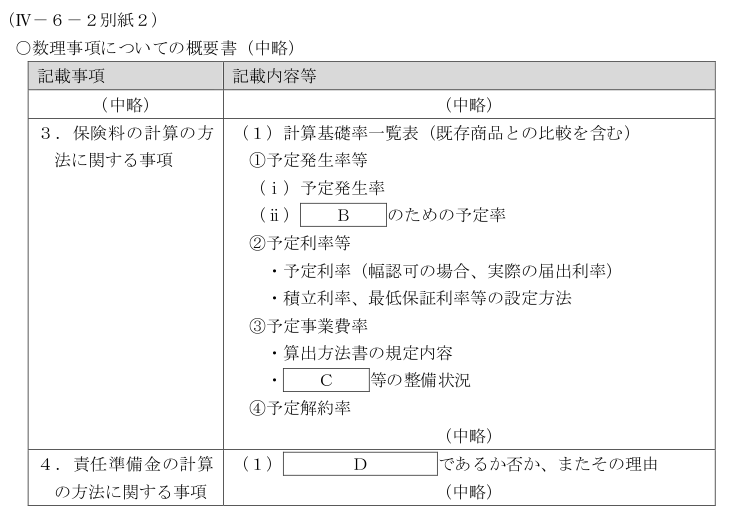
\includegraphics[scale=0.5]{./images/Prob2020-1-1-1-1.png}\\
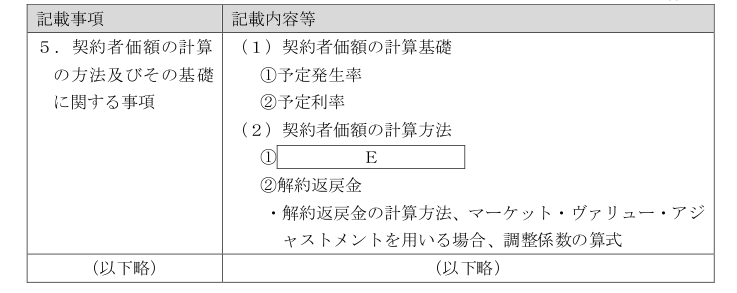
\includegraphics[scale=0.5]{./images/Prob2020-1-1-1-2.png}

\answer{}

\begin{itemize}
\item[ A:]  90 
\item[ B:]  保険料免除 
\item[ C:]  社内規定 
\item[ D:]  標準責任準備金対象契約 
\item[ E:]  保険契約上の責任準備金
\end{itemize}

\problem{2019 生保1問題 1(2)【監督指針】}
保険会社向けの総合的な監督指針「Ⅱ-2-5 商品開発に係る内部管理態勢」について、次の①~⑤に適切な語句を記入しなさい。

\noindent{}Ⅱ-2-5 商品開発に係る内部管理態勢\\
Ⅱ-2-5-1 意義

保険商品の内容は「普通保険約款」及び「\wakumaru{①}」に、料率については「\wakumaru{②}」に記載されてお
り、新商品の開発、商品内容の変更は、これらの変更を通じて行われている。

保険会社より商品の\wakumaru{③}申請が行われた場合、監督当局としては、契約内容が保険契約者等の
保護に欠けるおそれがないか、不当な差別的取扱いをするものではないか、契約内容が公序良俗を害
するものではないか等の保険業法に定める基準に適合するものであるか審査を行い、適当と認めら
れたものについて、これを\wakumaru{③}することとしている。

近年、保険商品には、わが国における社会の構造的変化・経済活動の多様化等に伴い、国民の生活
保障ニーズの高まり、新たなリスクの発生など、保険契約者ニーズに対応すべく多様化が求められて
いる。

こうしたニーズに応え、保険会社が商品開発を行うにあたっては、保険業法等の法令等を踏まえ、
\wakumaru{④}に基づき、リスク面、財務面、\wakumaru{⑤}、法制面等あらゆる観点から検討する内部管理態勢の整備が求められているところである。

\answer{}
\begin{itemize}
\item[ ① :] 事業方法書
\item[ ② :] 保険料及び責任準備金の算出方法書
\item[ ③ :] 認可
\item[ ④ :] 自己責任原則
\item[ ⑤ :] 募集面
\end{itemize}

\problem{2018 生保1問題 1(4)【監督指針】}

保険会社向けの総合的な監督指針「Ⅱ-2-5 商品開発に係る内部管理態勢」
「Ⅳ.保険商品審査上の留意点等」について、次のA〜Gに適切な語句を記入しなさい。

Ⅱ-2-5 商品開発に係る内部管理態勢

【省略】

Ⅱ-2-5-2 主な着眼点

(1)~(4)【省略】

(5)関連部門との連携

① ~ ②【省略】

③ 商品内容の概略決定にあたり、\wakumaru{A}、保険引受リスク、コンプライアンス、販売計画、システム開発、保険商品特有の道徳的危険等についての課題及び検討内容等を各関連部門において議論しているか。

なお、\wakumaru{A}については、商品ごとに保険会社の経営実態を踏まえた実現可能性の高い保険事故発生率並びに事業費その他のシナリオに基づき問題ないものとなっていることを確認しているか。

④ 社内規定等に定める付加保険料の算出方法が\wakumaru{B}かつ妥当なものであり、かつ、その算出された付加保険料が不当に差別的なものとなっていないことが確保されているか。特に、付加保険料の割増引きを設定する場合には、契約方法、保険料の払込方法等に基づいたものとなっており、事実上の\wakumaru{C}(法第 300 条第1項第5号)になっていないことに留意する。
【省略】

Ⅳ.保険商品審査上の留意点等

【省略】

Ⅳ-1 共通事項

第一分野、第二分野、第三分野の商品審査に係る共通事項として、特に以下の点に留意して審査することとする。

Ⅳ-1-1 普通保険約款及び特約の記載事項について

普通保険約款及び特約の記載事項については、\wakumaru{D}等の保護の観点から、明確かつ平易で、簡素なものとなっているかに留意することとする。

Ⅳ-1-2 保障又は補償の内容

\begin{itemize}
\item[ (1) ] 保障又は補償(以下、「保障等」という。)の内容が法第3条第4項から第6項に適合しているか。
\item[ (2) ] 保障等の内容が\wakumaru{D}等の\wakumaru{E}及び利便に適合しているか。
\item[ (3) ] 適正な死亡率や発生率が組み込まれているか、補償の内容が偶然性及び損害のてん補性を有しているかなど、\wakumaru{F}の有無に係る検討が十分行われているか。
\item[ (4) ] 支払事由に比して極端に高額な保険金が支払われるものや免責事由が極端に少ないもの、あるいは実損額を上回る保険金が支払われるものなどについては、射倖性が高いものとなっていたり、\wakumaru{G}が生じやすいものとなっていないか、検討が十分に行われているか。
\item[ (5) ] 支払事由が明確なものとなっているか。
\end{itemize}
【以下省略】
\answer{}
\begin{itemize}
\item[ A: ] 収支予測
\item[ B: ] 合理的
\item[ C: ] 特別利益の提供
\item[ D: ] 保険契約者
\item[ E: ] 需要
\item[ F: ] 保険性
\item[ G: ] モラルハザード
\end{itemize}

\problem{H29 生保1問題 1(1)【監督指針】}
保険会社向けの総合的な監督指針における団体保険又は団体契約の保険商品審査上の留意点につい
て、次の A~E に適切な語句を記入しなさい。

Ⅳ-1-14 団体保険又は団体契約の取扱い

団体保険又は団体契約については、以下の点に留意して審査することとする。

(1)団体及び被保険団体の範囲が、明確に定められているか。

(2)商品特性、募集管理態勢及び契約管理態勢、 A やリスク管理の状況等に照らし、 B
の排除や保険収支の安定等を目的として団体要件(例えば、一契約の最低被保険者数、 C
、最低加入率等)を定める必要がある場合、適切な団体要件を定めているか。
また、その場合に、被保険団体の区分(全員加入団体、任意加入団体)及び団体の区分に応じて、明確に定められているか。

(3)職域を基礎とする団体保険又は団体契約において、退職者及び退職者の配偶者等(以下、本項において「退職者等」という。)を引き続き被保険団体に含める場合は、以下の点を満たしているか。

① 団体が、退職者等に係る異動状況の把握及び保険料の収納管理を適切に行うための事務処理能力を有していること。
② 退職者等を被保険団体に含めること及び、これに伴って将来的に想定される退職者等の占める割合が
Dすることによる影響を踏まえ、A リスクに見合った保険料又は E 等の設定となっていること。

\answer{}
\begin{itemize}
\item[ A.] 保険引受 
\item[ B.] モラルリスク 
\item[ C.] 最高保険金額倍数 
\item[ D.] 上昇
\item[ E.] 配当方式
\end{itemize}

\problem{H27 生保1問題 1(1)【監督指針】}
保険会社向けの総合的な監督指針「Ⅳ-5 保険数理」について、次の①~⑦に適切な語句を記入しなさい。

\noindent{} Ⅳ-5 保険数理

算出方法書の審査にあたっては、特に以下の点に留意することとする。
\begin{itemize}
 \item [] Ⅳ-5-1 保険料\\
【省略】
 \item [] Ⅳ-5-2 責任準備金
\begin{enumerate}[(1)]
\item  (省略)
\item 商品の設計上、契約期間初期の給付を大きくすること若しくは将来の給付を減少させること又は
 保険料を後払いにすることについては、責任準備金が \wakumaru{①} とならないように設定されているか。
 なお、責任準備金の計算上、 \wakumaru{①} となる契約に係る責任準備金を \wakumaru{②} とする対応をとる場合
 においては、 \wakumaru{③} 確保に関する十分な検討がなされているかに留意する。
\item マーケット・ヴァリュー・アジャストメントの仕組みを持つ商品の責任準備金については、
\wakumaru{④} と \wakumaru{⑤} とのいずれか大きい額を積み立てることとなっているか。
\end{enumerate} 
\item [] Ⅳ-5-3 契約者価額\\
解約返戻金については、支出した\wakumaru{⑥}及び\wakumaru{⑦}の損失、保険設計上の仕組み等に照らし、合
理的かつ妥当に設定し、保険契約者にとって不当に不利益なものとなっていないか。
【以下省略】
\end{itemize}

\answer{}
\begin{itemize}
\item[ ①:]  負値
\item[ ②:]  ゼロ
\item[ ③:]  財務の健全性
\item[ ④:]  保険料積立金
\item[ ⑤:]  解約返戻金
\item[ ⑥:]  事業費
\item[ ⑦:]  投資上
\end{itemize}

\problem{H22 生保1問題 1(2)【監督指針】}
「保険会社向けの総合的な監督指針」に規定されている団体保険又は団体契約の商品審査上の留意
点について、以下の①~⑤の空欄に当てはまる適切な語句を答えなさい。

\begin{itemize}
\item[] 団体及び被保険団体の範囲が、明確に定められていること。
\item[] 被保険団体の区分(全員加入団体、任意加入団体)及び団体の区分(第Ⅰ種から第Ⅳ種等)に応じて、例えば一契約の\wakumaru{①}及び\wakumaru{②}が明確に定められていること。
\item[] 職域を基礎とする団体保険又は団体契約において、\wakumaru{③}及び\wakumaru{③}の配偶者等を引き続き被保険団体に含める場合、異動状況の把握及び保険料の収納管理を適切に行うための事務処理能力を有していること。
\item[]  \wakumaru{③}等を被保険団体に含めること及び、これに伴って将来的に想定される\wakumaru{③}等の占める割合が上昇することによる影響を踏まえ、保険引受リスクに見合った\wakumaru{④}又は\wakumaru{⑤}等の設定となっていること。
\end{itemize}

\answer{}
\begin{itemize}
\item[ ①: ] 最低被保険者数
\item[ ②: ] 最高保険金額倍数
\item[ ③: ] 退職者
\item[ ④: ] 保険料
\item[ ⑤: ] 配当方式
\end{itemize}

\problem{H21 生保1問題 2(1)【監督指針】}
保険金杜向けの総合的な監督指針における第三分野保険の基礎率変更権の設定について、以下の問に答えなさい。

①基礎率変更権行使基準の設定にあたっての満たすべき要件を挙げなさい。

②基礎率変更権の行使のための認可申請があった場合の審査の際の留意点を4っ挙げなさい。

\answer{}

\begin{itemize}
\item[①] 基礎率変更権行使基準の設定にあたって満たすべき要件
\begin{itemize}
\item[1)] 予定発生率に対する実績発生率の状況を示す指標については、予定発生率を変更して保険料又は保険金を変更するという趣旨に適合するものとして、次に掲げるいずれかの割合又は当該割合に準じたものとなっているか。
\begin{itemize}
\item[ア.] 予定発生率に対する実績発生率の割合
\item[イ.] 保険料収入(責任準備金繰入・戻入調整をした当該年度の危険保険料と付加保険料の合計)に対する保険金の支出額の割合
\end{itemize}
\item[2)] 1)に掲げる指標の設定にあたっては、実績発生率が悪化した場合の、当該保険契約の損益見込みに照らして、適切な水準となっているか。
\item[3)] 1)に掲げる指標に達した後、保険料又は保険金の変更を行う手続きが、明確になっているか。
\end{itemize}
\item[②] 第三分野保険の基礎率変更権の行使のための申請があった場合、審査上の留意事項
\begin{itemize}
\item[1)] 約款に定める基礎率変更権の規定(基礎率変更権行使基準等)に反しないものとなっているか。
\item[2)] 社内において定められている基礎率変更権の行使の手続きが遵守されているか。
\item[3)] 契約者に対して、契約締結時にあらかじめ十分な説明が行われ、その後も基礎率変更権行使基準に該当するかどうかの情報開示が定期的に行われていたか。
\item[4)] 変更後の予定発生率が、実績発生率等に照らして保険数理に基づく合理的かつ妥当なものとなっているか。
\end{itemize}
\end{itemize}

\problem{H18 生保1問題 1(1)【監督指針】}

金融庁の『保険会社向けの総合的な監督指針』のうち「Ⅳ保険商品審査上の留意点等 Ⅳ-5保険数
理」に規定されている、保険料及び責任準備金の算出方法書の審査に当たっての留意点のうち、保険料
に係わる項目(抜粋)について下記の空欄を埋めよ。

(1)保険料の算出方法については、 \wakumaru{①}や公平性等を考慮して、合理的かつ妥当なものとなっているか。

(2)保険料については、被保険者群団間及び保険種類間等で、不当な差別的扱いをするものとなっていないか。

(3)予定発生率・損害額又は予定解約率等については、基礎データに基づいて合理的に算出が行われ、かつ、基礎データの\wakumaru{②}に応じた補整が行われているか。(以下略)

(4)予定利率については、保険種類、保険期間、保険料の払方、運用実績や将来の利回り予想等を基に、合理的かつ\wakumaru{③}な観点から適切な設定が行われているか。

(5)(略)

(6)付加保険料(事業費の割増引を含む。)の設定について、係数によらずに定性的な表現で記載するときは以下の条件を満たしているか。

① 保険種類間の公平性が損なわれておらず、事業費の支出見込額に対して妥当であるなど適切なレベルとすることを明確にしているか。

② [Ⅱ-2-7-2(5)④] の主旨に則り、明確に社内規定等で定めることとしているか。

③ (1)(2)の観点を踏まえ、付加保険料の設定に応じ、その重要度を勘案した上で分類した保険種類及び\wakumaru{④}などの別ごとのに\wakumaru{⑤}を添付しているか。また、 \wakumaru{⑤}の基礎となる資料を添付しているか。(以下略)

\answer{}
\begin{itemize}
\item[ ①:] 十分性
\item[ ②:] 信頼度
\item[ ③:] 長期的
\item[ ④:] 販売経路
\item[ ⑤:] モニタリング資料
\end{itemize}

\problem{2022 生保2問題 1(1)【監督指針】}

「保険会社向けの総合的な監督指針」
【Ⅱ-2-1 責任準備金等の積立の適切性】について、以下
の(a)~(g)の空欄に当てはまる適切な語句または数値を記入しなさい。(7点)

\begin{itemize}
 \item [(ア)]「Ⅱ-2-1-2 積立方式(2)」においては以下が規定されている。\\
「第一分野及び第三分野において、保険会社の業務又は財産の状況及び保険契約の特性等
に照らし特別な事情がある場合に、保険数理に基づき、合理的かつ妥当なものとして、いわゆるチルメル式責任準備金の積立てを行っている場合には、 (a) に照らしチルメル歩合が妥当なものとなっているか。」
 \item [(イ)]「Ⅱ-2-1-2 積立方式(4)」においては以下が規定されている。\\
「特定の疾病による所定の状態、所定の身体障害の状態、所定の要介護状態その他の保険料
払込の免除事由に該当し、以後の保険料払込が免除されることとなった保険契約のうち、(b)の
可能な保険契約に係る責任準備金については、最終の保険期間満了日まで全て(b)が行われるものとして計算した金額を積み立てることとなっているか。」
\item[(ウ)]「Ⅱ-2-1-2 積立方式(5)」においては以下が規定されている。\\
「 (c) Ⅰ及びⅣにおける「 (d) 」に係る積立基準並びに積立限度の設定につい
ては、手術給付、介護給付その他の保険給付のリスクに応じたものとなっているか。
」
\item[(エ)]「Ⅱ-2-1-2 積立方式(7)④」においては以下が規定されている。\\
「ストレステスト及び (e) の基礎率を同じくする契約区分は同一のものを使用するこ
ととする。」
\item[(オ)]「Ⅱ-2-1-3-1 保険料積立金の積立(1)標準的方式①」においては以下が規定さ
れている。\\
「通常予測されるリスクに対応するものとして、標準的な計算式(
「一般勘定における最低
保証に係る保険金等の支出現価」から「一般勘定における最低保証に係る純保険料の収入現
価」を控除する形式の計算式)によって、概ね (f) %の事象をカバーできる水準に対
応する額を算出するものとなっているか。」
\item[(カ)]「Ⅱ-2-1-3-1 保険料積立金の積立(2)代替的方式④」において、平成8年2月
29日大蔵省告示第48号に列記する国内株式等の期待収益率及び (g) について、当
該告示に定めるものを使用する場合を除き、過去の実績や将来の資産運用環境の見通し、リ
スク中立の観点等から、合理的かつ客観的根拠に基づき定められる必要があることが規定
されている。
\end{itemize}
\answer{}
\begin{itemize}
\item[ (a): ] 新契約費水準
\item[ (b): ] 自動更新
\item[ (c): ] 危険準備金
\item[ (d): ] その他のリスク
\item[ (e): ] 負債十分性テスト
\item[ (f): ] 50
\item[ (g): ] ボラティリティ
\end{itemize}

\problem{2022 生保2問題 1(4)【監督指針】}
「保険会社向けの総合的な監督指針」
【Ⅱ-2-4 生命保険会社の区分経理の明確化】について、
以下の(a)~(e)の空欄に当てはまる適切な語句を記入しなさい。
(5点)

Ⅱ-2-4-2 主な着眼点

各生命保険会社においては、適切な区分経理を行うため、例えば、以下のような考えに基づく
区分経理に関する管理方針を策定しているか。また、区分経理の状況が、取締役会その他これ
に準ずる機関に対して報告されているか。

(1)〜(6) (省略)

(7)各区分間の取引等
\begin{itemize}
\item[①] 資産区分間の取引\\
資金移動(流入・流出)管理、 (a) 確保、ポートフォリオの改善等、必要な取引とし、市場価格等の適正な価格をもって適切に管理する。
\item[②]商品区分と全社区分との取引\\
\begin{itemize}
\item[ア.] 現預金等の貸借
\begin{itemize}
\item[(ア)] 商品区分又は全社区分毎に区別して管理する。
\item[(イ)] (b)が継続しないよう限度額等を設ける。
\end{itemize}
\item[イ.] 現預金等以外の貸借
\begin{itemize}
\item[(ア)]  (c) から (d) への貸付は、異常な保険金の支払い、新商品の販売に伴う事業運営資金、その他やむを得ない事情がある場合に限る。
\item[(イ)]  (d) から (c) への貸付は、 (c) の規模が小さいために、その機能を十分に果たすことができない場合に限る。
\item[(ウ)] 上記の貸借は、金額、利率(貸付期間に応じた市中金利等を基に設定すること)、期限その他の返済条件をあらかじめ定める。
\item[(エ)] 貸付条件の緩和や債務免除は、回収が不可能な損失が発生している場合等、やむを得ない事情がある場合を除き、 (e) 。なお、貸付条件の緩和等を行った後に利益が生じた場合は、当該利益を返済に充てるものとする。
\end{itemize}
\item[ウ.] 出資 (省略)
\item[エ.] その他の取引 (省略)
\end{itemize}
\end{itemize}

\answer{}
\begin{itemize}
\item[ (a): ]  流動性
\item[ (b): ]  借越し
\item[ (c): ]  全社区分
\item[ (d): ]  商品区分
\item[ (e): ]  行わない
\end{itemize}

\problem{2020 生保2問題 1(4)【監督指針】}
金融庁による事業費モニタリングについて、以下の①~⑤の空欄に当てはまる適切な語句を記入
しなさい。

\noindent ○「5-7\wakumaru{①}の充足状況」

保険種類・\wakumaru{②}
の区分ごとの新契約に係る事業費の効率等を見る資料で、定期的に
金融庁宛報告を要する。報告対象は、原則として、当該期における新契約の全て。

\wakumaru{①}に関して、保険種類および\wakumaru{②}の区分ごとに、
「\wakumaru{③}」、「事業費」、「\wakumaru{④}」を算出し、
「効率(事業費÷\wakumaru{③})」および「回収予定平均年数(事業
費÷\wakumaru{④})」を報告する。

\noindent ○「5-9 \wakumaru{⑤}の充足状況」

保険種類・\wakumaru{②}
の区分ごとの契約維持・管理のために支出する事業費の回収状況を
見る資料で、定期的に金融庁宛報告を要する。報告対象は、当該期における全保有契約。
\answer{}
\begin{itemize}
\item[ ①: ] イニシャルコスト
\item[ ②: ] 販売経路
\item[ ③: ] 予定事業費現価
\item[ ④: ] 年換算予定事業費
\item[ ⑤: ] ランニングコスト
\end{itemize}

\problem{2020 生保2問題 1(6)【監督指針】}
変額年金保険等の最低保証に係る保険料積立金の積立てに際して予定解約率を使用する場合の留
意点について、保険会社向けの総合的な監督指針の記載を踏まえ、簡潔に説明しなさい。

\answer{}
\begin{itemize}
\item[]  予定解約率が過去の実績や商品性等から、合理的に定められたものとなっているか。
\item[]  例えば、以下の事例等に留意しているか。
\begin{itemize}
\item[]  特別勘定の残高が最低保証額を下回る状態にあるときの解約率が、特別勘定の残高が最低保証額を超える状態にあるときの解約率より低い率となっているか。
\item[]  解約控除期間における解約率が、解約控除期間終了後の解約率と比べ、低い率となっているか。
\item[]  最低年金原資保証が付された保険契約で、年金開始前における特別勘定の残高が最低保証額を下回る状態にある場合において解約率を保守的に設定しているか。
\item[]  設定された予定解約率について、解約実績との比較などにより、検証を行うこととなっているか。
\end{itemize}
\end{itemize}

\problem{2019 生保2問題 1(1)【監督指針】}

「保険会社向けの総合的な監督指針」【Ⅱ-3-9 資産負債の総合的な管理】について、以下の
A~Eの空欄に当てはまる適切な語句を記入しなさい。

Ⅱ-3-9-1 意義

資産及び負債、資産の運用方針及び負債の管理方針が、AやBの状況に適
合していることを確保するためには、資産負債全体の状況を把握し管理するための効果的な態
勢を整備し、資産負債全体を適切に管理することが求められる。

Ⅱ-3-9-2 主な着眼点

\begin{itemize}
 \item[(1): ]  (省略)
 \item[(2): ]  取締役会は、資産負債全体の総合的な管理に関する戦略目標を設定し、戦略目標の中でCに関する方針を明確化しているか。
 \item[(3): ]  (省略)
 \item[(4): ]  (省略)
 \item[(5): ]  資産負債を統合的に管理する際に、少なくとも、Dに対する潜在的な影響に関して重要と考えられるリスクは資産負債管理の枠組みにおいて評価されているか。なお、そのようなリスクとしては以下のリスクが含まれる。
 \item[①: ] 市場リスク(省略)
 \item[②: ] 保険引受リスク
 \item[③: ] リスク
\end{itemize}

(以下、省略)
\answer{}
\begin{itemize}
\item[ A: ] リスクの特性
\item[ B: ] ソルベンシー
\item[ C: ] リスク許容度
\item[ D: ] 経済価値
\item[ E: ] 流動性
\end{itemize}
\problem{2018 生保2問題 1(3)【監督指針】}
保険会社向けの総合的な監督指針」【Ⅱ-2-4 生命保険会社の区分経理の明確化】につい
て、以下のA~Eの空欄に当てはまる適切な語句を記入しなさい。

Ⅱ-2-4-1 意義 (省略)

Ⅱ-2-4-2 主な着眼点

各生命保険会社においては、適切な区分経理を行うため、例えば、以下のような考えに基づ
く区分経理に関する管理方針を策定しているか。また、区分経理の状況が、取締役会その他
これに準ずる機関に対して報告されているか。

(1)~(4) (省略)

(5) 資産の配賦方法及び管理基準
\begin{itemize}
\item[①] 運用資産の配賦方法\\
運用資産は、原則として、資産の購入時に配賦する資産区分を決める。
\item[②] 運用資産の管理\\
運用資産は、資産区分ごとに、次に掲げる方式の中から適切な方式を選択し管理する。
\item[ア.: ] A・・・ 個々の資産を銘柄ごとに、資産区分に直接帰属させる方式
\item[イ.: ] B・・・ 取引単位(例えば、不動産では物件ごと)ごとに、資産区分の持分で管理する方式
\item[ウ.: ]  資産持分管理方式・・・ 投資対象資産ごとのマザーファンドを設定し、各資産のマザーファンドに対する持分を管理する方式
(注)資産持分管理方式を用いる場合は、一般勘定資産(C保険に対応する資産を除く。)全体を一個のマザーファンドとして扱わない。
\item[③] 運用資産以外の配賦方法\\
再保険貸等、各資産区分に直課できるものは直課し、直課できないものは、区分経理に関
する管理方針に基づいて配賦する。
\item[④] 全社区分の資産\\
D、子会社・関連会社株式、E(E等の管理機能を持つ場合)、その他全社区分に配賦することが相応しい資産の全部又は一部を配賦するものとする。
\end{itemize}
(6)、(7) (省略)

Ⅱ-2-4-3 監督手法・対応 (省略)

\answer{}
\begin{itemize}
\item[ A: ] 資産分別管理方式
\item[ B: ] 資産単位別持分管理方式
\item[ C: ] 無配当
\item[ D: ] 営業用不動産
\item[ E: ] 現預金
\end{itemize}

\problem{H29 生保2問題 1(6)【監督指針】}
「保険会社向けの総合的な監督指針」【Ⅱ-3-5 リスクとソルベンシーの自己評価】につ
いて、以下の①~⑥の空欄に当てはまる適切な語句を記入しなさい。

Ⅱ-3-5-1 意義

保険会社は、経営戦略及びリスク特性等に応じ、自らのリスク管理の適切性と現在及び将来
にわたるソルベンシーの十分性を評価するために、①の責任の下、定期的にリスクとソルベンシーの自己評価を実施することが求められる。自己評価においては、将来の経済状況や他の外部要因の変化も考慮し、合理的に予見可能で関連性のある重大なリスクを含んでいる必要がある。

Ⅱ-3-5-2 リスクとソルベンシーの自己評価

(1) 保険会社は、将来の経済状況やその他の外部要因の変化を含めた合理的に予見可能で関
連性のある全ての重大なリスクを考慮し、資本の②と十分性の評価を実施している
か。

また、リスクの要因やリスクの重要性の程度を定期的に評価しているか。さらに、③に大きな変化があった場合には、速やかにリスクとソルベンシーの再評価を行っているか。

保険会社は、リスクとソルベンシーの自己評価に当たっては、中長期事業戦略(例えば3年から5年間)、特に新規事業計画に十分留意しているか。

(2) 保険会社は、必要な④及びソルベンシー・マージン規制に基づく資本の要件を満たしているかをモニタリングするために、リスクとソルベンシーの自己評価を定期的に行い、リスクと資本の管理プロセスを整備しているか。また、必要な④とソルベンシー・マージン規制に基づく資本の要件の違いについて、経営陣は適切に認識しているか。

(3) 保険会社は、リスクとソルベンシーの自己評価の結果を、例えば、リスクの特定及び③、リスク測定、リスク管理方針及びリスクとソルベンシーの自己評価の結果を踏まえた行動計画等とともに、適切に⑤しているか。

(4) 保険会社は、リスクとソルベンシーの自己評価の有効性について、内部(例えばリスク管理担当役員など)又は外部による全般的な評価を行っているか。

(5) ⑥部門は、統合的リスク管理及びリスクとソルベンシーの自己評価の有効性を独立した立場から検証し、必要に応じ経営陣に提言を行っているか。

Ⅱ-3-5-3 経営計画とソルベンシー評価

(1)、(2) (省略)

\answer{}
\begin{itemize}
\item[ ①: ]  取締役会
\item[ ②: ]  質
\item[ ③: ]  リスク・プロファイル
\item[ ④: ]  経済資本
\item[ ⑤: ]  文書化
\item[ ⑥: ]  内部監査
\end{itemize}

\problem{H28 生保2問題 1(3)【監督指針】}
ストレステストについて、以下の①〜⑤の空欄に当てはまる適切な語句を記入しなさい。

「保険会社向けの総合的な監督指針」の II -3-3-3 ストレステスト

保険会社は、将来の不利益が①に与える影響をチェックし、必要に応じて、追加的に
経営上又は財務上の対応をとって行く必要がある。そのためのツールとして、
②等を含むストレステスト(想定される将来の不利益が生じた場合の影響に関する分析)及び
③(経営危機に至る可能性が高いシナリオを特定し、そのようなリスクをコントロール
すべく必要な方策を準備するためのストレステスト)が重要である。特に、市場が大きく変動し
ているような状況下では、④によるリスク管理には限界があることから、ストレステストの活用は極めて重要である。保険会社においては、⑤等も勘案しつつ、財務内容及び
保有するリスクの状況に応じたストレステストを自主的に実施することが求められる。

\answer{}

\begin{itemize}
 \item[①] 財務の健全性
 \item[②] 感応度テスト
 \item[③] リバース・ストレステスト
 \item[④] VaR
 \item[⑤] 市場の動向
\end{itemize}

\problem{H28 生保2問題 1(4)【業法, 監督指針】}
金融庁による事業費モニタリングについて、以下の①〜⑤の空欄に当てはまる適切な語句を記入しなさい。

○生命保険会社は、平成18年4月以降、次の5つの資料を金融庁宛定期報告することとなっている。
\begin{itemize}
\item[ ・]  5−5「予定事業費等の設定状況」
\item[ ・]  5−6「総合的な充足状況」
\item[ ・]  5−7「①の充足状況」
\item[ ・]  5−8「①の回収状況」
\item[ ・]  5−9「②の充足状況」
\end{itemize}

○5-7「①の充足状況」について
保険種類および③の区分ごとの新契約に係る事業費の効率等を見る資料で、定期的に金融庁宛報告を要する。報告対象は、原則として、当該期における新契約の全て。

①に関して、保険種類および③の区分ごとに、「④」、「事業費」、「⑤」を算出し、
「効率(事業費÷④)」および「回収予定平均年数(事業費÷⑤)」を報告する。
\answer{}
\begin{itemize}
\item[① : ] イニシャルコスト
\item[② : ] ランニングコスト
\item[③ : ] 販売経路
\item[④ : ] 予定事業費現価
\item[⑤ : ] 年換算予定事業費
\end{itemize}

\problem{H23 生保2問題 2(1)【監督指針,実務基準】}
区分経理の意義および商品区分の設定について、「保険会社向けの総合的な監督指針」および「保険検査マニュアル」の内容を踏まえ、簡潔に説明しなさい。

\answer{}

\noindent ○区分経理の意義.
\begin{itemize}
\item[] 生命保険会社においては、利益還元の公平性・透明性の確保、保険種類相互間の内部補助の遮
 断、事業運営の効率化、商品設計や価格設定面での創意工夫などを図る観点から、一般勘定に
 ついて保険商品の特性に応じた区分経理を行うことが重要である。
\item[] 各生命保険会社において自己責任原則のもと、保険経理の透明性、保険契約者間の公平性確保
 等の観点から、適切な区分経理が行われる必要がある。
\item[] また、区分経理を導入するにあたっては、資産の配分方法、含み損益の配賦方法等について、
 アセットシェア等に基づき適切に配分方法が定められていることが重要である。
\item[] なお、区分経理は保険計理人の確認業務(責任準備金に関する事項、剰余金の分配または契約
 者配当に関する事項)にも関連している。
\end{itemize}
\noindent ○商品区分の設定
\begin{itemize}
\item[] 区分経理を活用する上では、その目的に応じた適切かつ有効な区分を設定することが重要であ
 り、保険の性質の相違等により理論的かつ合理的な区分とする必要がある。したがって、会社
 収支に重大な影響を与える場合等は、商品区分の新設や細分化をして管理することが望ましい。
 ただし、期間損益の安定性や事務負荷等を踏まえて重要性を検討した上で導入することが重要
 である。また、設定した商品区分については、商品ポートフォリオが大きく変化する場合等に
 は設定を見直す必要もある。
\item[] 保険検査マニュアルには、次のような留意点が記載されている。
\begin{itemize}
\item[①] 商品区分は、損益及び負債の管理を行うためのものであるが、商品の特性や契約の保有状況
に照らして、損益を把握する単位として適切なものとなっているか。\\
 例えば、「掛捨型の短期保険と貯蓄型の長期保険」、「無配当保険と有配当保険」、「予
 定利率固定型保険と予定利率変動型保険」、「個人保険と企業保険」などが、原則として、
 別区分で管理されているか。\\
 なお、主契約に付加された特約等は、原則として、主契約と同じ商品区分に帰属させてい
 るか。
\item[②] 新規商品の発売による当該保有契約の増大や、ある商品区分の中の一部の保険種類の契約
 の増大などにより、保険会社全体や商品区分の収支に重大な影響を与えるような場合に、
 新たな商品区分又は同種の細分化した商品区分を設定する際に、契約者間の公平性等に留意し、
合理的な方法で行っているか。
\item[③] 設定した商品区分について、合理的な理由(保有契約が減少し、商品区分の存在意義がな
 くなった場合等)がないにもかかわらず、その変更(他の商品区分に統合することを含
 む。)を行っていないか。
\end{itemize}
\end{itemize}
\noindent ○活用方法および留意点

\begin{itemize}
 \item[] 利益還元の公平性・透明性の確保
\begin{itemize}
\item[] 区分経理を行うことで、区分毎の損益の状況を明確にすることが可能となるため、利益還元の
 公平性・透明性を確保することができる。特に、有配当区分における契約者への配当の公平性・
 透明性を確保するために、有配当契約・無配当契約を区分するといった適切な区分経理の実施
 は重要である。
\item[] 法令では、剰余金の分配または契約者配当の計算は、
 「保険契約の特性に応じて設定した区分ご
 とに」計算することが規定されており、また、生命保険会社の保険計理人の実務基準では、公
 正・衡平な配当の確認における商品区分単位の配当可能財源の確認は「区分経理の商品区分毎
 に」行うことと規定されている。
\end{itemize}
 \item[] 保険種類相互間の内部補助の遮断
\begin{itemize}
\item[] 商品区分はセルフサポートが基本であり、その中で保険料および責任準備金の十分性を満たす
 必要がある。言い換えれば、区分毎の十分性の確保が、契約者間の公平性の確保および会社の
 健全性の確保につながる。特に、生命保険会社の保険計理人の実務基準では、責任準備金の十
 分性確認において区分経理の商品区分毎に将来収支分析を行うことと規定されている。
\item[] ただし、区分経理は現状ではあくまで内部管理会計であることもあり、最終的には全体で支払
 能力を裏付けていることにも留意する。
\item[] 商品区分の規模が小さくなると、分散効果の低下により毎年の保険収支が不安定化したり資産
 運用効率が低下したりすることから、安定的・効率的な保険制度の運営が難しくなる。このこ
 とから、無闇・頻繁な区分の変更は当然避けられるべきではあるが、一方で、発売間もない新
 商品の区分や販売停止して長期間経つなどして保有が減少した商品の区分など、小さすぎる区
 分は、他の商品区分への統合も検討するなど、区分の更新を検討する必要がある。また、この
 ような目的のために厳格な貸借・出資を前提として全社区分を活用することも考えられる。
\end{itemize}
 \item[] 事業運営の効率化
\begin{itemize}
\item[] 区分経理を行うことで、区分毎の効率性を把握することが可能となり、不採算区分の事業規模
 縮小・撤退などを検討する上での有効な判断材料となる。さらに、その区分の特性を把握でき、
 手数料などの販売政策、経営資源投入などの経営戦略の策定が可能となる。
\item[] 商品に対応する資産の運用特性に沿った区分とすることで、資産運用の効率性・資産負債マッ
 チングの向上や責任準備金対応債券の効果的な運用など、ALM を効果的に行うことができる。
\item[] 区分経理を行う上で算定・利用される保険関係収支などの各種の情報やインフラはリスク管理
 にも利用することができる。
\item[] 分析を行う上でも経営上の諸作を行う上でも区分経理が有効に働くように、商品特性・資産運
 用特性などに沿った商品区分とすることが必要である。例えば、配当の有無・保証性または貯
 蓄性・外貨建かどうかなどによって区分することは必要であろう。
\item[] ただし、区分経理の商品区分に基づく分析だけでなく、保険種類毎や販売チャネル毎など、更
 に細分化した分析や、単年度損益に加え、エンベディッドバリューや新契約価値などの評価手
 法を併用するなど、多面的な分析を行った上で経営判断に役立てていくことが重要である。
\item[] 区分毎の効率性を把握するためには事業費の配賦が不可欠ではあるが、間接経費の詳細な配賦
 は一般的に困難である。これらはあくまでも配賦によって得られた数字であり、常に精度改善
 の余地を持つことに留意が必要である。
\item[] また、一般に、細分化には情報収集コスト・インフラ整備が必要であり、費用対効果に留意が
 必要である。
\item[] 区分経理を効果的に経営に反映させるためにも、経営陣の区分経理に対する理解促進を図るこ
 と・アクチュアリー自身の説明能力の向上を図ることが必要である。
\end{itemize}
 \item[] 商品設計や価格設定面での創意工夫などを図る
\begin{itemize}
\item[] 例えば、独立した商品区分及び資産区分を設定することにより、利率変動型商品や外貨建商品
 などのような資産運用結果を契約者価額に反映させた商品の開発が可能となる。
\item[] また、他の金融商品に競合する商品を開発する場合には、資産区分の資産運用方針に基づき予
 定利率を定め、必要ならば解約返戻金を市場価格調整型とすることで、リスクコントロールを
 しつつ、魅力ある商品設計が可能になる。
\item[] 利源分析を区分毎に行うことで、計算基礎率の妥当性のチェックなどのより詳細な分析を行う
 こともでき、これを新商品開発時の計算基礎率に反映することができる。特に、商品区分別の
 事業費を把握し、それを保険種類別・販売チャネル別に按分することでそれぞれの保険種類・
 販売チャネルに必要な予定事業費率を把握することができるようになる。
\end{itemize}
\end{itemize}

\problem{H22 生保2問題 2(1)【監督指針】}
保険契約を再保険に付した場合の責任準備金の不積立てについて、関連する法令および「保険会社向けの総合的な監督指針」における記載も踏まえ、簡潔に説明しなさい。

\answer{}
再保険に付した契約であっても、保険事故が発生した場合、保険金受取人からの請求に対して責
任を負うのは元受保険会社であり、再保険していることにより免責となるわけではない。受再会社
が破綻した場合のことを考慮すれば、再保険に付した部分も含めて元受保険会社が責任準備金を積
み立てることも考えられる。ただ、この場合、再保険方式によっては、元受保険金杜に過度な負担
を強いることになる。

このため、保険業法施行規則において、保険会社等に出再する場合は、健全な出再先への出再と
して、再保険を付した部分に相当する責任準備金を積み立てないことができるとされている。
また、「保険金杜向けの総合的な監督指針」においては、この取扱いの可否について、当該再保
険契約がリスクを将来にわたって確実に移転する性質のものであるかどうかや、当該再保険契約に
係る再保険金等の回収の蓋然性が高いかどうかに着目して判断すべきであるとされ、回収の蓋然性
の評価にあたっては、少なくとも再保険契約を引き受けた保険会社又は外国保険業者の財務状況に
ついて、できる限り詳細に把握する必要がある、とされている。

生命保険の再保険として代表的なものに、共同再保険方式や毎年の危険保険金部分を再保険する
方式があるが、これらの再保険に付した契約における責任準備金については、前者の場合は、保険
料、保険金等の全ての契約者との金銭を再保険割合に応じて分かち合うことになるため、責任準備
金も元受会社と再保険金杜で再保険割合に応じて積み立てなければ、収支に歪みが生ずることにな
る。一方、後者の場合は、元受保険金杜から再保険金杜に支払う再保険料も、貯蓄部分を含まない
その年の危険保険料に対応したものとなっており、この場合は、再保険金杜に必要な責任準備金は、
定期保険や一般の損害保険に近い方式のものであり、元受保険会社の保険料積立金から、出再部分
を控除することはできず、未経過保険料の出再分を控除することができる。

\problem{H22 生保2問題 2(4)【監督指針】}

保険会社向けの総合的な監督指針において、財務の健全性に関するリスク管理でのストレステス
トの実施を定めているが、生命保険会社がストレステストを行う意義およびストレスシナリオの設
定において留意すべき点について、監督指針に沿って簡潔に説明しなさい。
\answer{}
\begin{itemize}
\item[①] 生命保険会社がストレステストを行う意義
\begin{itemize}
\item[・] 保険会社は、将来の不利益が財務の健全性に与える影響をチェックし、必要に応じて、追加的に経営上又は財務上の対応をとって行く必要がある。そのためのツールとして、感応度テスト等を含むストレステスト(想定される将来の不利益が生じた場合の影響に関する分析)は重要である。
\item[・] 特に、市場が大きく変動しているような状況下では、VaRによるリスク管理には限界があることから、ストレステストの活用は極めて重要である。
\item[・] 保険会社においては、市場の動向等も勘案しつつ、財務内容及び保有するリスクの状況に応じたストレステストを自主的に実施することが求められる。
\end{itemize}
\item[②] ストレスシナリオの設定において留意すべき点
\begin{itemize}
\item[・] ヒストリカルシナリオ(過去の主な危機のケースや最大損失事例の当てはめ)のみならず、仮想のストレスシナリオによる分析も行っているか。
\item[・] 仮想のストレスシナリすについては、内外の経済動向に関し、株式の価格、金利、為替、信用スプレッドなど、保険会社の保有するリスクに応じて、複数の要素についてストレスシナリオを作成しているか。
\item[・] 複数の要素が同時に変動するシナリオについて、前提となっている保有資産間の価格の相関関係が崩れるような事態も含めて検討を行っているか。
\item[・] 保有する資産の市場流動性が低下する状況を勘案しているか。
\item[・] 変額年金保険の様なオプション・保証性の高い要素については、その特性を考慮した上で、適切なストレスシナリオを設定しているか。
\item[・] 再保険やデリバティブ等によるリスクのヘッジを行っている場合には、カウンターパーティリスクを考慮してストレスシナリオを設定しているか。
\item[・] ストレステストの設定に際しては、取締役会において、保険会社におけるリスク管理の方針として、基本的な考え方を明確に定めているか。
\item[・] その際、基本的な考え方は、統合リスク管理との間に矛盾がなく、かつ、統合リスク管理の計量化手法で把握できないリスクを捉えるとの観点からの配慮がなされているか
\item[・] また、取締役会等において、定期的に、かつ必要に応じ随時、保険会社の業務の内容等を踏まえ、設定内容を見直しているか。等
\end{itemize}
\end{itemize}

\problem{H20 生保2問題 1(2)【監督指針】}
\begin{itemize}
\item[・] 区分経理は、内部管理会計として行っている状況であるが、「保険会社向けの総合的な監督指針」(金融庁)には、一区分経理の明確化として内容が規定されている。
\item[・] 会社の損益等を区分する単位として、①及び②を設定する。①については、損益を把握する単位として適切なものとなっている必要があり、保険の性質の相違等により理論的・合理的な区分とする必要がある。②には例えば次のイから二の機能がある。
\begin{itemize}
\item[イ.] 死亡保障リスク等の③機能
\item[口.] 新商品開発に係る事業運営資金提供機能
\item[ハ.] 会社全体で共有する資産・共通する経費等の管理機能
\item[二.] 現預金等の管理機能
\end{itemize}
\item[・]運用資産は、資産区分ごとに、資産分別管理方式・④方式・⑤方式の中から適切な管理方式を選択し管理する。
\end{itemize}

\answer{}
\begin{itemize}
\item[①:] 商品区分
\item[②:] 全社区分
\item[③:] リスクバッファー
\item[④:] 資産単位別持分管理
\item[⑤:] 資産持分管理(またはマザーファンド)
\end{itemize}
※④と⑤は1頃不同


\subsection{施行規則}

\problem{2022 生保1問題 1(1)【施行規則】}
保険業法施行規則第 10 条について、次の①~⑤に適切な語句を記入しなさい。(5点)

第 10 条(\wakumaru{①}の記載事項)

免許申請者は、法第3条第4項の生命保険業免許の申請の場合にあっては第1号から第6号まで及び第8号に掲げる事項を、
(略)法第4条第2項第4号に掲げる書類に記載しなければならない。

\begin{itemize}
\item[ 一  ] 保険料の計算の方法(略)に関する事項
\item[ 二  ] 責任準備金(法第\wakumaru{②}条第1項の責任準備金をいう。(略))の計算の方法(略)に関する事項
\item[ 三  ] 返戻金の額その他の被保険者のために積み立てるべき額を基礎として計算した金額(以下「\wakumaru{③}」という。)の計算の方法及びその基礎に関する事項
\item[ 四  ] 第 30 条の5第1項第1号の社員配当準備金又は第 64 条第1項の契約者配当準備金及び社員に対する剰余金の分配又は契約者配当の計算の方法に関する事項
\item[ 五  ] \wakumaru{④}の計上に関する事項
\item[ 六  ] 保険金額、保険の種類又は\wakumaru{⑤}を変更する場合における計算の方法に関する事項
\item[ 七  ]( 略)
\item[ 八  ] その他保険数理に関して必要な事項
\end{itemize}

\answer{}
\begin{itemize}
\item[ ① ] 保険料及び責任準備金の算出方法書 
\item[ ② ] 116 
\item[ ③ ] 契約者価額 
\item[ ④ ] 未収保険料
\item[ ⑤ ] 保険期間
\end{itemize}

\problem{H28 生保1問題 1(1)【業法,施行規則】}
以下の保険業法および保険業法施行規則の抜粋について、次の①~⑤に適切な語句を記入しなさい。

【保険業法第3条(免許)】\\
【省略】

4.生命保険業免許は、第1号に掲げる保険の引受けを行い、又はこれに併せて第2号若しくは第3号に掲げる保険の引受けを行う事業に係る免許とする。
\begin{itemize}
\item[ 一 ] 人の\wakumaru{①}(当該人の …【中略】… 同じ。)に関し、一定額の保険金を支払うことを約し、保険料を収受する保険(次項ハに …【中略】… を除く。)
\item[ 二 ] 次に掲げる事由に関し、一定額の保険金を支払うこと又はこれらによって生ずることのある当該人の損害をてん補することを約し、保険料を収受する保険
\begin{itemize}
\item[ イ ] 人が\wakumaru{②}にかかったこと。
\item[ ロ ] \wakumaru{③}を受けたこと又は\wakumaru{②}にかかったことを原因とする人の状態
\item[ ハ ] \wakumaru{③}を受けたことを直接の原因とする人の死亡
\item[ ニ ] イ又はロに掲げるものに類するものとして内閣府令で定めるもの(人の死亡を除く。)
\item[ ホ ] イ、ロ又はニに掲げるものに関し、治療(治療に類する …【中略】… を含む。)を受けたこと。
\end{itemize}
\item[ 三 ] 次項第1号に掲げる保険のうち、再保険であって、前2号に掲げる保険に係るもの
 【省略】
\end{itemize}

【保険業法施行規則第4条(\wakumaru{②}等に類する事由)】

法第3条第4項第2号二に規定する内閣府令で定める事由は、次に掲げる事由とする。

\begin{itemize}
\item[ 一 ]  \wakumaru{④}及びこれを原因とする人の状態
\item[ 二 ]  \wakumaru{⑤}を要する身体の状態
\item[ 三 ]  老衰を直接の原因とする常時の介護を要する身体の状態
\item[ 四 ]  骨髄の提供及びこれを原因とする人の状態
\end{itemize}

\answer{}
\begin{itemize}
\item[ ①: ]  生存又は死亡
\item[ ②: ]  疾病
\item[ ③: ]  傷害
\item[ ④: ]  出産
\item[ ⑤: ]  不妊治療
\end{itemize}

\problem{H26 生保1問題 1(1)【施行規則】}
保険業法施行規則において生命保険会社が「保険料及び責任準備金の算出方法書」 に記載しなけれ
ばならないとされる事項について、次の①~⑤の空欄に当てはまる適切な語句を記入しなさい。

\begin{itemize}
\item[ ] 保険料の計算の方法に関する事項
\item[ ] 責任準備金の計算の方法に関する事項
\item[ ] \wakumaru{①}の額その他の被保険者のために積み立てるべき額を基礎として計算した金額の計算の方法及びその基礎に関する事項
\item[ ] 社員配当準備金又は\wakumaru{②}準備金及び社員に対する剰余金の分配又は\wakumaru{②}の計算の方法に関する事項
\item[ ] \wakumaru{③}の計上に関する事項
\item[ ] 保険金額、保険の種類又は\wakumaru{④}を変更する場合における計算の方法に関する事項
\item[ ] その他\wakumaru{⑤}に関して必要な事項
\end{itemize}

\answer{}
\begin{itemize}
\item[①:]  返戻金
\item[②:]  契約者配当
\item[③:]  未収保険料
\item[④:]  保険期間
\item[⑤:]  保険数理
\end{itemize}

\problem{H25 生保1問題 1(3)【施工規則】}
保険業法施行規則第71条および大蔵省告示第233号(平成10年6月8日)によって定義され
ている財務再保険について以下の①~③の空欄に当てはまる適切な語句を答え、下の表の各欄に
A~Cを埋めなさい。

\begin{tabular}{|l|c|c|c|}
 \hline
\multirow{2}{*}{}& \multicolumn{2}{c|}{将来収益に基づいた手数料を元受会社が受けるもの}
 &\multirow{2}{*}{その他}\\  \cline{2-3}
&告示第233号第1号の要件をすべて満たすもの&その他&\\ \hline
共同保険式  & & & \\ \hline
修正共同保険式 & & & \\ \hline
その他 & & & \\ \hline
\end{tabular}

\begin{itemize}
\item[ A:] 日本の法令上、「財務再保険」と定義されることにより、 \wakumaru{①}を\wakumaru{②}することができる。
\item[ B:] 日本の法令上、「財務再保険」と定義されないことにより、 \wakumaru{①}を\wakumaru{②}できず、 \wakumaru{③}として計上しなければならない。
\item[ C:] 日本の法令上、何の規制もない。
\end{itemize}
\answer{}

\begin{itemize}
\item[ ①: ] 手数料収入
\item[ ②: ] 収益認識
\item[ ③: ] 預かり金
\end{itemize}

\begin{tabular}{|l|c|c|c|}
 \hline
\multirow{2}{*}{}& \multicolumn{2}{c|}{将来収益に基づいた手数料を元受会社が受けるもの}
 &\multirow{2}{*}{その他}\\  \cline{2-3}
&告示第233号第1号の要件をすべて満たすもの&その他&\\ \hline
共同保険式  & A&B &C \\ \hline
修正共同保険式 &A &B & C \\ \hline
その他 & B & B & C\\ \hline
\end{tabular}

\problem{H15 生保1問題 1(3)【施工規則】}
以下は、保険業法施行規則第 10 条(保険料及び責任準備金の算出方法書の記載事項)の要点を抄出
したものである。空白部分にあてはまる適切な文言を選択肢より選んで解答せよ。

「免許申請者は、法第 3 条第 4 項の生命保険業免許の申請の場合にあっては第 1 号から第 6 号まで
及び第 9 号に掲げる事項を、同条第 5 項の損害保険業免許の申請の場合にあっては第 1 号から第 4 号
まで及び第 6 号から第 9 号までに掲げる事項を、法第 4 条第 2 項第 4 号に掲げる書類に記載しなけれ
ばならない。

\begin{itemize}
\item[ 一]  \wakumaru{①} の計算の方法(その計算の基礎となる係数を要する場合においては、その係数を含む。) に関する事項
\item[ 二]  \wakumaru{②} (法第百十六条第一項の \wakumaru{②} をいう、以下この章から第八章までにおいて同じ。)の 計算の方法(その計算の基礎となる係数を要する場合においては、その係数を含む。)に関する 事項
\item[ 三]  \wakumaru{③} の額その他の \wakumaru{④} のために積み立てるべき額を基礎として計算した金額の計算の方 法及びその基礎に関する事項
\item[ 四]  第 28 条第 1 項第 1 号の社員配当準備金又は第 64 条第 1 項の契約者配当準備金及び社員に対する剰余金の分配又は契約者配当の計算の方法に関する事項
\item[ 五]  \wakumaru{⑤} の計上に関する事項
\item[ 六]  保険金額、保険の種類又は保険期間を変更する場合における計算の方法に関する事項
 (以下略) 」
\end{itemize}

〔選択肢〕\\
a 未経過保険料 b 保険契約者 c 未収保険料d 保険料e 危険準備金\\
f 支払備金 g 返戻金 h 責任準備金 i 契約者価額 j 被保険者
\answer{}

\begin{itemize}
\item[ ① ] d 保険料
\item[ ② ] h 責任準備金
\item[ ③ ] g 返戻金
\item[ ④ ]  j 被保険者
\item[ ⑤ ] c 未収保険料
\end{itemize}

\problem{H13 生保1問題 1(3)【施行規則】}
財務再保険の取り扱いは保険業法施行規則第71条第2項および平成10年大蔵省告示
第233号に規定されているが、これに関して次の①〜⑤を適当な語句で埋めよ。

財務再保険とは、元受会社が保有する保険契約に係る\wakumaru{①}のリスクを移転する
再保険契約であって、当該保険契約から将来にわたって発生することが見込まれる収
益を\wakumaru{②}としてあらかじめ一定額を収受するものをいい(ただし、ある一定の条件を
満たす必要がある)、元受会社は\wakumaru{②}の金額を\wakumaru{③}として積み立てる。財務再保
険の種類は\wakumaru{④}式再保険と\wakumaru{⑤}式再保険の2種類がある。

\answer{}
\begin{itemize}
\item[ ①: ] すべて
\item[ ②: ] 出再保険受入手数料(初年度コミッション)
\item[ ③: ] 責任準備金
\item[ ④: ] 共同保険
\item[ ⑤: ] 修正共同保険
\end{itemize}

〔解説〕以下のような根拠規定によって問題文は組み立てられている。
\begin{itemize}
\item[ ・]  保険業法71条第2項「…手数料を収受したときは、当該収受した金額を\underline{責任準備金}として積み立てなければならない。」
\item[ ・]  平成10年大蔵省告示第233号第1条「…当該再保険に付した部分に係る\underline{すべて}のリスクを移転することを約し、当該再保険に付した部分に係る保険契約から当該再保険に付した後に発生することが見込まれる収益を\underline{出再保険受入手数料}としてあらかじめ収受する再保険であって…」
\item[ ・]  同第2条第1項「財務再保険の種類は、次に掲げる二種類とする。\\
 一 \underline{共同保険}式再保険 二 \underline{修正共同保険}式再保険」
\end{itemize}

\problem{H28 生保2問題 1(2)【施行規則】}

生命保険会社の保険計理人の関与事項について、以下の①~⑤の空欄に当てはまる適切な語句
を記入しなさい。

生命保険会社の保険計理人の関与事項は、次に掲げるものに係る①に関する事項である。

\begin{itemize}
\item[ 1]  保険料の算出方法
\item[ 2]  ②の算出方法
\item[ 3]  契約者配当又は社員に対する剰余金の分配に係る算出方法
\item[ 4]  ③の算出方法
\item[ 5]  未収保険料の算出
\item[ 6]  ④の算出
\item[ 7]  ⑤に関する計画
\item[ 8]  生命保険募集人の給与等に関する規程の作成
\item[ 9]  その他保険計理人がその職務を行うに際し必要な事項
\end{itemize}
\answer{}
\begin{itemize}
\item[ ① ] 保険数理
\item[ ② ] 責任準備金
\item[ ③ ] 契約者価額
\item[ ④ ] 支払備金
\item[ ⑤ ] 保険募集
\end{itemize}

\problem{H26 生保2問題 1(1)【業法, 施行規則】}

各種準備金に関する次の①~⑤の文章について、下線部分が正しい場合は○、誤っている場合
は×を記入するとともに、誤っている場合には下線部分を正しい表現に改めなさい。

① 保険業法第56条では、基金を償却(基金拠出者への返済)するときは、その償却する金額に相当する金額を、\underline{基金償却準備金}として積み立てなければならないと規定されている。

② 価格変動準備金の積立限度に関して、対象資産のうち国内法人発行の株式については、\underline{期末市場価額}に 100/1000 を乗じて計算する。

③ 危険準備金Ⅱの取崩しにあたっては、\underline{逆ざや}がある場合において、当該\underline{逆ざや}のてん補に充てるときを除くほか、取り崩してはならない。

④ 保険業法施行規則第30条の5で規定される\underline{社員配当準備金}とは、社員への剰余金分配の額を安定させるために積み立てる任意積立金である。

⑤ 生命保険株式会社の経理処理において、契約者配当準備金繰入額は\underline{費用処理}される。

\answer{}
\begin{itemize}
\item[ ①: ] ×基金償却積立金
\item[ ②: ] ×期末帳簿価額
\item[ ③: ] ×利差損
\item[ ④: ] ×社員配当平衡積立金
\item[ ⑤: ] ○
\end{itemize}

\problem{H24 生保2問題 1(2)【業法,施行規則】}

生命保険相互会社における剰余金の分配に関し、以下の①~⑤の空欄に当てはまる適切な語句
を記入しなさい。

・保険業法第55条の2では「剰余金の分配は、①な分配をするための基準として内閣府令で定める基準に従い、行わなければならない。」と定めている。「内閣府令で定める基準」として、保険業法施行規則第30条の2で以下のとおり規定している。

・相互会社が社員に対する剰余金の分配をする場合には、②に応じて設定した区分ごとに、剰余金の分配の対象となる金額を計算し、次の各号に掲げるいずれかの方法により、又はそれらの方法の併用により行わなければならない。

1.社員が支払った保険料及び保険料として収受した金銭を運用することによって得られる収益から、保険金、返戻金その他の給付金の支払、事業費の支出その他の費用等を控除した金額に応じて分配する方法(③方式)

2.剰余金の分配の対象となる金額をその発生の原因ごとに把握し、それぞれ各保険契約の責任準備金、保険金その他の基準となる金額に応じて計算し、その合計額を分配する方法(④方式)

3.剰余金の分配の対象となる金額を⑤等により把握し、各保険契約の責任準備金、保険料その他の基準となる金額に応じて計算した金額を分配する方法

4.その他前三号に掲げる方法に準ずる方法

\answer{}
\begin{itemize}
\item[ ①: ] 公正かつ衡平
\item[ ②: ] 保険契約の特性
\item[ ③: ] アセット・シェア
\item[ ④: ] 利源別配当
\item[ ⑤: ] 保険期間
\end{itemize}

\problem{H18 生保2問題 1(2)【施行規則】}
保険業法施行規則第六十九条(生命保険会社の責任準備金)について、以下の空欄を埋めよ。

第六十九条(生命保険会社の責任準備金)

生命保険会社は、毎決算期において、次の各号に掲げる区分に応じ、当該決算期以前に収入した①を基礎として、当該各号に掲げる金額を法第四条第二項第四号に掲げる書類に記載された方法に従って計算し、責任準備金として積み立てなければならない。

一 ②

保険契約に基づく将来の債務の履行に備えるため、③に基づき計算した金額(第二号の二の払戻積立金として積み立てる金額を除く。)

二 ④

未経過期間(保険契約に定めた保険期間のうち、決算期において、まだ経過していない期間をいう。次条及び第二百十一条の四十六において同じ。)に対応する責任に相当する額として計算した金額(次号の払戻積立金として積み立てる金額を除く。)

二の二 払戻積立金 (省略)\\
三 危険準備金 (省略)\\
2〜5(省略)

6 第一項第三号の危険準備金は、次に掲げるものに区分して積み立てなければならない。

一 第八十七条第一号に掲げる保険リスクに備える危険準備金\\
二 同条第二号に掲げる予定利率リスクに備える危険準備金\\
三 同条第二号の二に掲げる⑤に備える危険準備金
(省略)

7 (省略)
\answer{}

\begin{itemize}
\item[ ①:] 保険料
\item[ ②:] 保険料積立金
\item[ ③:] 保険数理
\item[ ④:] 未経過保険料
\item[ ⑤:] 最低保証リスク
\end{itemize}


\subsection{業法}
\problem{2022 生保2問題 1(2)【業法】}
生命保険会社の保険計理人の職務(保険業法第121条)について、以下の(a)~(e)の空
欄に当てはまる適切な語句を記入しなさい。
(5点)

\begin{itemize}
\item[(ア)] 保険計理人は、毎決算期において、次に掲げる事項について、内閣府令で定めるところにより確認し、その結果を記載した(a)を(b)に提出しなければならない。
\begin{itemize}
\item[・]  内閣府令で定める保険契約に係る責任準備金が (c) に基づいて積み立てられているかどうか。
\item[・]  契約者配当又は社員に対する剰余金の分配が(d)に行われているかどうか。
\item[・]  その他内閣府令で定める事項
\end{itemize}
\item[(イ)] 保険計理人は、(ア)の(a)を(b)に提出した後、遅滞なく、その写しを(e)に提出しなければならない。
\item[(ウ)] (e)は、保険計理人に対し、(イ)の(a)の写しについてその説明を求め、その他その職務に属する事項について意見を求めることができる。
\item[(エ)] 上記に定めるもののほか、(ア)の(a)に関し必要な事項は、内閣府令で定める。
\end{itemize}

\answer{}
\begin{itemize}
\item[ (a): ] 意見書
\item[ (b): ] 取締役会
\item[ (c): ] 健全な保険数理
\item[ (d): ] 公正かつ衡平
\item[ (e): ] 内閣総理大臣
\end{itemize}
※(e)は「金融庁(長官)」も正答とした。

\problem{H14 生保1問題 1(2)【業法】}
生命保険業免許は保険業法第3条第4項に規定されている。同規定に関して次の①〜⑤を適当な語句で埋めよ。

「生命保険業免許は、第一号に掲げる保険の引受けを行い、又はこれに併せて第二号若しくは第三号に掲げる保険の引受けを行う事業に係る免許とする。

\begin{itemize}
\item[一: ] 人の\wakumaru{①}(当該人の余命が一定の期間以内であると医師により診断された身体の状態を含む。以下この項及び次項において同じ。)に関し、\wakumaru{②}の保険金を支払うことを約し、保険料を収受する保険(次号ハに掲げる死亡のみに係るものを除く。)
\item[二: ] 次に掲げる事由に関し、[重コの保険金を支払うこと又はこれらによって生ずることのある当該人の損害をてん補することを約し、保険料を収受する保険
\item[イ: ] 人が疾病にかかったこと。
\item[口: ] \wakumaru{③}を受けたこと又は疾病にかかったことを原因とする人の状態
\item[ハ: ] \wakumaru{③}を受けたことを直接の原因とする人の死亡
\item[ニ: ] イ又は口に掲げるものに類するものとして内閣府令で定めるもの(人の死亡を除く。)
\item[ホ: ] イ、口又は二に掲げるものに関し、\wakumaru{④}(\wakumaru{④}に類する行為として内閣府令で定めるものを含む。)を受けたこと。
\item[三: ] 次項第一号に掲げる保険のうち、\wakumaru{⑤}であって、前二号に掲げる保険に係るもの」
\end{itemize}

\answer{}
\begin{itemize}
\item[ ①: ] 生存又は死亡
\item[ ②: ] 一定額
\item[ ③: ] 傷害
\item[ ④: ] 治療
\item[ ⑤: ] 再保険
\end{itemize}



\subsection{その他; 大蔵省告示, 保険法}

\problem{H28 生保1問題 1(2)【大蔵省告示】}
大蔵省告示第233号(平成10年6月8日)について、次の①~⑤に適切な語句を記入しなさい。

第1条(財務再保険)

保険業法施行規則(以下「規則」という。)第71条第2項に規定する金融庁長官が定める再
保険は、保険会社が保険契約を再保険に付した場合において、当該再保険に付した部分に係る
\wakumaru{①}を移転することを約し、当該再保険に付した部分に係る保険契約から当該再保険に付
した後に発生することが見込まれる収益(以下 …【中略】… という。)を
\wakumaru{②}(受再 …【中略】… 同じ。)としてあらかじめ収受する再保険であって、次に掲げるすべての要件に該
当するものをいう。

一 【省略】\\
二 元受保険会社が受再保険会社から収受する\wakumaru{②}は\wakumaru{③}によるものであること。\\
三 【省略】\\
四 受再保険会社による\wakumaru{④}は、元受保険会社の再保険料の不払いによる場合を除き、できないものであること。
【省略】

第2条(種類)\\
【第1項省略】

2.前項第1号に掲げる\wakumaru{⑤}とは、受再保険会社が、元受保険契約(元受保険会社 …【中略】… 同じ。)に係るリスクのうち、当該再保険に付された部分に係る\wakumaru{①}を出再割合(受再保険会社 …【中略】… 同じ。)に応じて引き受け、当該引き受けた部分に係る責任準備金(保険業法 …【中略】… 同じ。)の積立て及び当該責任準備金に相当する額の資産の管理を行うものをいう。
【以下省略】

\answer{}
\begin{itemize}
\item[ ①: ]  すべてのリスク
\item[ ②: ]  出再保険受入手数料
\item[ ③: ]  現金
\item[ ④: ]  一方的な解約
\item[ ⑤: ]  共同保険式再保険
\end{itemize}


\problem{H24 生保1問題 1(3)【保険法】}
保険法に規定されている保険契約について、次の①~⑥の空欄に当てはまる適切な語句を答えなさい。

\begin{itemize}
\item[ ・ ] 生命保険契約とは、保険契約のうち、保険者が人の①又は②に関し一定の③を行うことを約するもの(傷害疾病定額保険契約に該当するものを除く。)をいう。
\item[ ・ ] 損害保険契約とは、保険契約のうち、保険者が一定の④によって生ずることのある損害を⑤することを約するものをいう。
\item[ ・ ] 傷害疾病定額保険契約とは、保険契約のうち、保険者が人の傷害疾病に基づき一定の③を行うことを約するものをいう。
\item[ ・ ] 傷害疾病損害保険契約とは、⑥のうち、保険者が人の傷害疾病によって生ずることのある損害(当該傷害疾病が生じた者が受けるものに限る。)を⑤することを約するものをいう。
\end{itemize}

\answer{}
\begin{itemize}
\item[ ① ]  生存
\item[ ② ]  死亡
\item[ ③ ]  保険給付
\item[ ④ ]  偶然の事故
\item[ ⑤ ]  てん補
\item[ ⑥ ]  損害保険契約
\end{itemize}

\problem{H21 生保1問題 1(1)【大蔵省告示】}
次の再保険に関する説明文について、以下の①~⑦の空欄に適切な語句を解答用紙の所定の欄に記
入しなさい。

\begin{itemize}
\item[] 平成 10 年 大蔵省告示第 233 号においては、再保険契約のうち、元受会社が出再部分についてす
 べてのリスクを移転し、出再部分からの将来収益を出再保険受入手数料として収受するもので、か
 つ同告示第 1 条ならびに第 2 条の条件を同時に満たすものを\wakumaru{①}として定義している。
 この場合、手数料収入を\wakumaru{②}することができる。

\item[] 将来収益を出再保険受入手数料として収受するものであっても、同告示第 1 条ないし第 2 条の条
 件のうち少なくとも一つを満たさない再保険契約については、\wakumaru{①}とは認められない。
 この場合、手数料収入を\wakumaru{②}することができず、
 \wakumaru{③}として計上しなければならない。

\item[] この規制の趣旨は、元受会社が再保険を活用して収益の発生するタイミングを早期化することに
 伴う、将来の\wakumaru{④}にかかわるリスクをコントロールすることにある。

\item[] 集積リスクの規模や性質により、再保険会社だけでは引き受けられない場合、資本市場にリスクを
 移転するために、保険リスクを証券化したものを\wakumaru{⑤}と呼ぶ。

\item[] この証券化のために、\wakumaru{⑥}を設立し、この\wakumaru{⑥}が再保険会社となって、
 元受会社から保険リスク(Cat Cover)を引き受ける一方、\wakumaru{⑥}が資本市場において
 \wakumaru{⑤}を発行し、このCat Coverのリスクを\wakumaru{⑥}から投資家に移転する。
 \wakumaru{⑤}は、Cat Coverの保険事故が発生した場合、元受会社に再保険金を支払う原資として償還金
 や利息の一部または全部が支払われない一方で、そのリスクの対価として、\wakumaru{⑦}への上乗せが行
 われる。
\end{itemize}

\answer{}
\begin{itemize}
\item[ ①: ] 財務再保険
\item[ ②: ] 収益認識(「収益計上」も可)
\item[ ③: ] 預かり金
\item[ ④: ] 責任準備金(積み立て)不足
\item[ ⑤: ] カタストロフィーボンド(「Catボンド」も可)
\item[ ⑥: ] 特定目的会社(「SPC」も可)
\item[ ⑦: ] 利率
\end{itemize}

\problem{2021 生保2問題 1(4)【税制】}
生命保険会社の税制について、以下の①~⑤の空欄に当てはまる適切な語句または数値を記入し
なさい。

\begin{itemize}
\item[・] 責任準備金繰入額については、保険料積立金及び未経過保険料の部分に限り、保険料及び責
任準備金の算出方法書に定められている\wakumaru{①}の計算基礎を基として計算した額を限度
として損金算入できる。ただし、
\wakumaru{②}の対象契約については、平成8年の大蔵省告示
第48号に定められた計算基礎を基として計算した額を損金算入限度額とすることができる。
\item[・] 法人事業税(地方税)の課税標準は、生命保険業にあっては各事業年度の収入金額とされて
おり、生命保険業の各事業年度の収入金額は、収入保険料中の\wakumaru{③}相当額とするとの
考え方から、収入保険料に一定割合を乗じた金額と定められている。なお、法人事業税の一
部を分離した地方法人特別税は令和元年9月30日までに開始する事業年度をもって廃止さ
れた一方で、令和元年10月1日以後に開始する事業年度から\wakumaru{④}(国税)が創設さ
れている。
\item[・] 課税所得が当該事業年度の剰余金の額の\wakumaru{⑤}相当額に満たない場合は、契約者(社員)
配当準備金繰入額の損金算入を制限し、この剰余金の\wakumaru{⑤}相当額を課税標準とする制
度が設けられている。
\end{itemize}
\answer{}
\begin{itemize}
\item[ ①: ] 保険料
\item[ ②: ] 標準責任準備金
\item[ ③: ] 付加保険料
\item[ ④: ] 特別法人事業税
\item[ ⑤: ] 7%
\end{itemize}


\problem{H29 生保2問題 1(1)【大蔵省告示】}

平成10年・大蔵省告示第231号に規定されている、危険準備金の取崩基準について、以
下の①~⑤の空欄に当てはまる適切な語句を記入しなさい。

(危険準備金の取崩基準)

第六条 危険準備金Ⅰ及び危険準備金Ⅳは、それぞれ①がある場合において、当該
①のてん補に充てるときを除くほか、取り崩してはならない。

2 危険準備金Ⅱは、②がある場合において、当該②のてん補に充てるときを除くほか、取り崩してはならない。

3 危険準備金Ⅲは、最低保証に係る③が負の場合において、当該③のてん補に充てるときを除くほか、取り崩してはならない。

4 その他前三項それぞれに共通する取崩基準として、前事業年度末の④の額が当該事業年度末の⑤を超える場合は、当該超える額を取り崩さなければならない。

\answer{}
\begin{itemize}
\item[ ①: ] 死差損
\item[ ②: ] 利差損
\item[ ③: ] 収支残
\item[ ④: ] 積立残高
\item[ ⑤: ] 積立限度額
\end{itemize}

\problem{H27 生保2問題 1(5)【大蔵省告示】}
平成 8 年・大蔵省告示第 50 号別表第 6 の 2 に規定されている、変額年金保険等の最低保証リス
ク相当額の算出について、次のA~Eに適切な語句を記入しなさい。

II. 最低保証リスク相当額の算出
\begin{itemize}
\item[1.] 標準的方式
\begin{itemize}
\item[(1)]最低保証リスク相当額は、次のイに掲げる額からロに掲げる額を控除した額とする。
\begin{itemize}
\item[イ]Aの責任準備金の額(原則として法第 4 条第 2 項第 4 号に掲げる書類に記載された商品区分ごとに、次の①から④までに定める手順に基づき算出した額をいう。)
\begin{itemize}
\item[①] 次に掲げる区分に応じたリスク対象資産の額から、別表第 7 の 2 の区分によるそれぞれの対象取引残高の欄に掲げる額(別表第 7 の 2 によりリスクヘッジの有効性が確認できたものに限る。)を控除した残高に、次の表に掲げる区分に応じた下落率をそれぞれ乗じた額の合計額を算出する。(省略)
\item[②] 上記①に掲げる額から、その額に次に掲げる算式により計算したB係数を乗じた額を控除する。(省略)
\item[③] 上記②により算出した額を特別勘定資産の額の合計額で除した率を算出する。
\item[④] 上記③により算出した率に基づき資産下落が生じたとした場合の、一般勘定におけるCの額を算出する。
\end{itemize}
\item[ロ] 法第 4 条第 2 項第 4 号に掲げる書類に記載された方法に基づき算出された一般勘定におけるCの額
\item[(2)] (省略)
\item[(3)] (省略)
\item[2.] 代替的方式
次の①から⑬に定める基準を満たす保険会社、外国保険会社等又は免許特定法人(以下「保険会社等」という。)は代替的方式を用いることができる。ただし、代替的方式を用いた場合は、Dの結果、代替的方式の使用を継続することが不適当と認められ、代替的方式の使用を中断する旨又はEに重大な変更を加える旨をあらかじめ金融庁長官に届け出た場合を除き、これを継続して使用しなければならない。(以下、省略)
\end{itemize}
\end{itemize}
\end{itemize}
\answer{}
\begin{itemize}
\item[ A: ] 資産価格下落後
\item[ B: ] 分散投資効果
\item[ C: ] 最低保証に係る責任準備金
\item[ D: ] バック・テスティング
\item[ E: ] リスク計測モデル
\end{itemize}

\problem{H18 生保2問題 2(1)【大蔵省告示】}
平成8年・大蔵省告示第48号第5項に規定されている、変額年金保険等の最低保証に係る保険
料積立金の積立方式である「標準的方式」を簡潔に説明せよ。また、それを使用する場合における留
意点を挙げ、金融庁の「保険会社向けの総合的な監督指針」の記載内容を踏まえ簡潔に説明せよ。(10点)

\answer{}
<「標準的方式」の内容について>

「標準的方式」により計算される保険料積立金は次の①から②を控除した金額である。\\
①一般勘定における最低保証に係る保険金等の支出現価\\
②一般勘定における最低保証に係る純保険料の収入現価

<「標準的方式」を使用する場合における留意点>

[全般]: 通常予測されるリスクに対応するものとして、標準的な計算式によって、概ね
50%の事象をカバーできる水準に対応する額を算出するものとする。

[予定死亡率]: 最低死亡保険金保証が付された保険契約においては死亡保険用の標準死
亡率を、最低年金原資保証が付された保険契約については年金開始後用の標準死亡率を、
両方の保証が付された保険契約においては、保険料積立金の積立が保守的となる方の標
準死亡率を使用する。

[割引率]: 割引率として標準利率を使用する。

[期待収益率]: 期待収益率として標準利率を使用する。

[ボラティリティ]: 資産種類に応じて以下のボラティリティを使用する。なお、下記以
外の資産種類のボラティリティに関しては過去の実績等から合理的に定めたものを使
用する。\\
国内株式:18.4%、邦貨建債券:3.5%、\\
外国株式:18.1%、外貨建債券:12.1%

[予定解約率]: 以下の点に留意したうえで、過去の実績や商品性等から合理的に定める。\\
特別勘定の残高が最低保証額を下回る状態にあるときの解約率が、特別勘定の残高
が最低保証額を超える状態にあるときの解約率より低い率とする。\\
解約控除期間における解約率が、解約控除期間終了後の解約率と比べ、低い率とする。\\
最低年金原資保証が付された保険契約で、年金開始前における特別勘定の残高が最
低保証額を下回る状態にある場合において解約率を保守的に設定する。\\
設定した予定解約率について、解約実績との比較などにより、検証を行う。

[その他の基礎率]: 過去の実績や商品性等から合理的に設定する。

\problem{H17 生保2問題1(2)改題【大蔵省告示】}

平成 8 年・大蔵省告示第 48
号に規定されている予定利率(標準利率)の水準の設定について、以下の空欄を適切な語句または数値で埋めよ。④については計算過程も記載せよ。

<平成 11 年 4 月 1
日以降の標準利率の水準の設定の概要\textbf{(平準払保険の場合)}> 毎年
10 月 1 日を基準日として、基準日の属する月の前月から過去①年間または過去
10 年間に発行された利付国庫債券(10
年)の応募者利回りのそれぞれの平均値のいずれか②い方の値を下表に掲げる対象利率に区分して、それぞれの数値に安全率係数を乗じて得られた数値の合計値(基準利率)が、基準日時点で適用されている予定利率と比較して③\%以上乖離している場合には、基準利率に最も近い
0.25%の整数倍の利率(基準利率が 0.25%の整数倍の利率と
0.125%乖離している場合は、基準利率を超えず、かつ、基準利率に最も近い
0.25%の整数倍の利率とする。)を予定利率とし、基準日の翌年の 4 月 1
日以降締結する保険契約に適用する。

\begin{longtable}[]{@{}ll@{}}
\toprule
対象利率 & 安全率係数\tabularnewline
\midrule
\endhead
0%を超え、1.0%以下の部分 & 0.9\tabularnewline
1.0%を超え、2.0%以下の部分 & 0.75\tabularnewline
2.0%を超え、\textbf{4.0%}以下の部分 & 0.5\tabularnewline
\textbf{4.0%}を超える部分 & 0.25\tabularnewline
\bottomrule
\end{longtable}

<標準利率の水準の計算> 平成 11 年以降のある年の 4 月 1
日時点で適用されている標準利率を
1.50%とする。同年の基準日の属する月の前月から過去に
①年間の利付国庫債券(10 年)の応募者利回りの平均値が 2.90\%、過去 10
年間の応募者利回りの平均値が 4.25%とすると、その翌年の 4 月 1
日以降締結する保険契約の標準利率の水準は④\%となる。
※上記\textbf{強調部}が現行規制との整合のため修正した箇所

\answer{解答}

①3 ②低 ③0.5 ④1×0.9+1×0.75+0.9×0.5=2.10(1.50と0.5以上乖離)→2.0%

%%%%%%%%%%%%%%%%%%%



\end{document}
